%
% Complete documentation on the extended LaTeX markup used for Insight
% documentation is available in ``Documenting Insight'', which is part
% of the standard documentation for Insight.  It may be found online
% at:
%
%     http://www.itk.org/

\documentclass{InsightArticle}

\usepackage{graphicx}

%%%%%%%%%%%%%%%%%%%%%%%%%%%%%%%%%%%%%%%%%%%%%%%%%%%%%%%%%%%%%%%%%%
%
%  hyperref should be the last package to be loaded.
%
%%%%%%%%%%%%%%%%%%%%%%%%%%%%%%%%%%%%%%%%%%%%%%%%%%%%%%%%%%%%%%%%%%
\usepackage[bookmarks,bookmarksopen,backref,colorlinks,linkcolor={blue},citecolor={blue},urlcolor={blue}]{hyperref}


%  This is a template for Papers to the Insight Journal. 
%  It is comparable to a technical report format.

% The title should be descriptive enough for people to be able to find
% the relevant document. 
\title{Local Shape Analysis using MANCOVA}

% 
% NOTE: This is the last number of the "handle" URL that 
% The Insight Journal assigns to your paper as part of the
% submission process. Please replace the number "1338" with
% the actual handle number that you get assigned.
%
\newcommand{\IJhandlerIDnumber}{1338}
\newcommand{\ProgramName}{\textit{shapeAnalysisMANCOVA}}

% Increment the release number whenever significant changes are made.
% The author and/or editor can define 'significant' however they like.
\release{0.00}

% At minimum, give your name and an email address.  You can include a
% snail-mail address if you like.
\author{Beatriz Paniagua, Martin Styner, Marc Macenko, Dimitrios Pantazis and Marc Niethammer}

\authoraddress{The University \textit{of} North Carolina \textit{at} Chapel Hill}

\begin{document}

%
% Add hyperlink to the web location and license of the paper.
% The argument of this command is the handler identifier given
% by the Insight Journal to this paper.
% 
\IJhandlefooter{\IJhandlerIDnumber}
\maketitle


\ifhtml
\chapter*{Front Matter\label{front}}
\fi


% The abstract should be a paragraph or two long, and describe the
% scope of the document.
\begin{abstract}
\noindent

Gross shape measures such as volume have been widely used in statistical analysis of anatomical structures. Statistical shape analysis methods have emerged within the last decade to allow for a localized analysis of shape. Most shape analysis frameworks are though lacking a good statistical underpinning, as they commonly do not allow for the inclusion of independent variables such as age, gender or clinical scores.

This work presents a unified method for local shape analysis that can accomodate different number of variates and contrasts. It also allows to include any number of associated variables in the statistical analysis of the data. Several cases of study are given to clarify the explanation of the different types of data that can be analyzed and the parameters that can be used to tune the program \ProgramName. This tool has been designed to interact seamlessly with the existing UNC SPHARM-PDM \cite{Styner06} based shape analysis toolbox.
\end{abstract}

\IJhandlenote{\IJhandlerIDnumber}

\tableofcontents

\section{Introduction}
\label{sec:intro}

Quantitative shape features such as volumetric measurements have been widely used in statistical shape analysis of diverse anatomical structures in previous years. Volume changes are intuitive features as they might explain morphological variation due to illness, but structural local changes at specific locations are not sufficiently reflected in volume measurements. Shape analysis has thus become of increasing interest due to its potential to precisely locate morphological changes between healthy and pathological structures. One of the first and most influential research in shape analysis was presented by D’Arcy \cite{Thompson42} in his ground-breaking book \textit{On Growth and Form}. In more recent years, several researchers proposed shape analysis via medial shape computing and analysis using M-rep \cite{Styner03}. Medial shape analysis separately analyzes the two medial shape properties: local position and thickness \cite{Styner03_2}. However, this analysis methods were not corrected for multiple, correlated statistical tests. \cite{Pizer99}, and Golland \cite{Golland99} proposed shape analysis on medial shape descriptions in 3D and 2D, respectively. They used a fixed topology sampled model with implicit correspondence that is fitted to the objects. Another set of studies can be found on shape analysis via deformable registration to a template (\cite{Davatzikos96}, \cite{Joshi97}, \cite{Csernansky98}, \cite{Csernansky02}). In this studies, inter-subject comparisons are made by analyzing the individual deformable transformations. This analysis of the transformation fields has to cope with the high dimensionality of the transformation, the template selection problem and the sensitivity to the initial position. 

All of these studies are focused in local analysis of specific areas of the structures, via multivariate analysis, but have mostly lacked the ability to include independent clinical variables in that analysis. The work presented in this paper offers statistical shape analysis based on a parametric boundary description (SPHARM \cite{Brechbuhler95}) as the point-based model computing method. The point-based models will be analyzed with the methods here proposed using multivariate analysis of covariance (MANCOVA). Here, the number of variates being tested is the dimensionality of our observations. Each point of these observations is a three dimensional displacement vector from the mean. The number of contrasts is the number of equations involved in the null-hypothesis. In order to encompass varying numbers of variates and contrasts, and to account for independent variables, a matrix computation is performed. This matrix represents the multidimensional aspects of the correlation significance and it can be transformed into a scalar measure by manipulation of its eigenvalues. The various ways of combining these eigenvalues is discussed in section \ref{sec:stats}. Section \ref{sec:linearmodel} describes the linear model framework used in the analysis, while section \ref{sec:stats} describe the statistical methods applied. Section \ref{sec:program} describes \ProgramName   usage as well as the input and outputs associated. Finally, sections \ref{sec:results} and \ref{sec:conclusions} present several analysis scenarios in detail and the results and conclusions obtained, respectively. 

\section{Traditional Approach}
\label{sec:tradapproach}

After correspondence establishment using SPHARM-PDM \cite{Brechbuhler95} \cite{Styner06}, alignment and scaling normalization in a shape population, the traditional statistical analysis approach  consisted in testing for differences between groups at every surface location. The steps performed in order to obtain the statistical analysis are shown in figure \ref{fig:tradflow}.

\begin{figure}[htbp]
  \begin{center}
    \begin{tabular}[htbp]{c}
    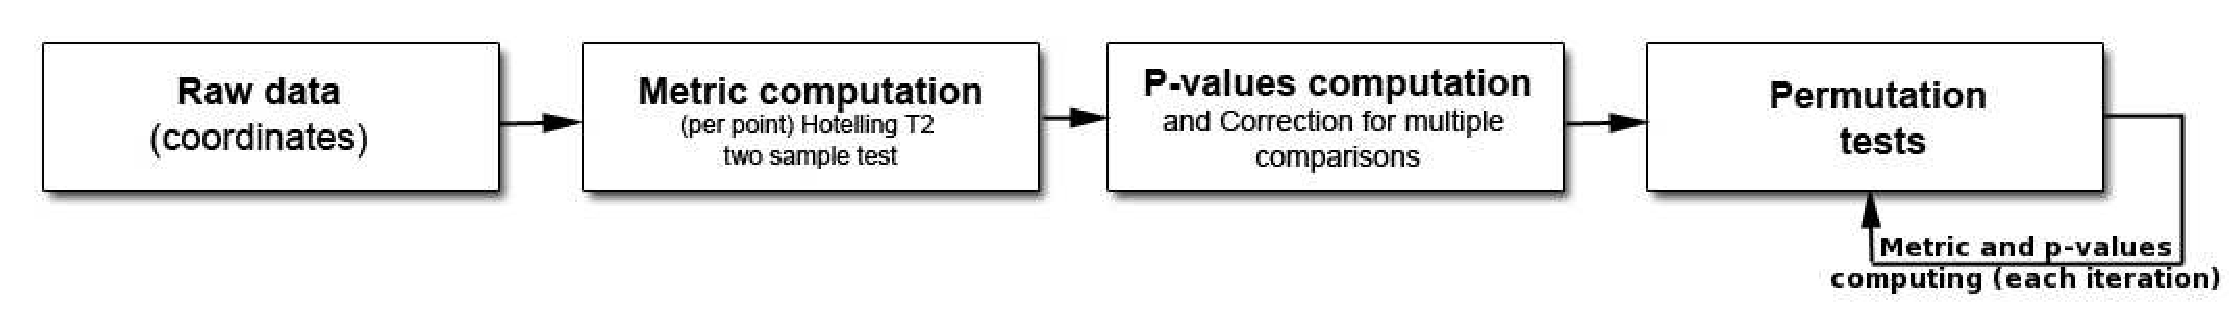
\includegraphics[width=0.9\textwidth]{IJ_TraditionalAp}
    \end{tabular}
    \itkcaption{Workflow used in the previous used approach for statistical analysis.}
    \label{fig:tradflow}
  \end{center}
\end{figure}

In the following sections each one of these steps will be seen in detail.

\subsection{Local Testing of Group Mean Difference using Hotelling $T^2$ metric}
\label{sec:TestMethods}

In the previous statistical framework, it was possible to test for differences between two shape populations in two main fashions:

\begin{itemize}
\item \emph{Analyzing the magnitude of the local difference vector to a template:} For this option, a template needs to be first selected, usually this template is the common mean of the two groups or the mean of a separate control group.  The magnitude of the difference is easily understood and results in difference maps for each subject. Also, the resulting univariate statistical analysis is quite well known and local significance can be easily computed using the Student t metric. The main disadvantage of this method is the need to select a template, which introduces an additional bias into the statistical analysis. We applied this method in earlier studies of hippocampi \cite{Styner04MedIA} and ventricles \cite{Styner05PNAS}.
\item \emph{Analyzing the spatial location of each point:} For this option, no template is necessary and multivariate statistics of the $(x,y,z)$ location is necessary. We have chosen to use the Hotelling $T^2$ two sample difference metric as a measurement of how two groups locally differ from each other. The standard Hotelling $T^2$ is defined as 
$T^2 = (\mu_1 - \mu_2)' (\Sigma (\frac{1}{n_1} + \frac{1}{n_2}))^{-1} (\mu_1 - \mu_2)$, where $\Sigma = (\Sigma_1 (n_1 -1) + \Sigma_2 (n_2 -1))/ (n_1 +n_2 -2)$ is the pooled covariance matrix. An alternative modified Hotelling $T^2$ metric is less sensitive to group differences of the covariance matrixes and the number of samples\cite{Seber04}: $T^2 = (\mu_1 - \mu_2)' (\Sigma_1 \frac{1}{n_1} + \Sigma_2 \frac{1}{n_2})^{-1} (\mu_1 - \mu_2)$. All our current studies are based on this modified Hotelling $T^2$ metric.
\end{itemize}

\begin{figure}[htbp]
  \begin{center}
    \begin{tabular}[htbp]{c|c}
      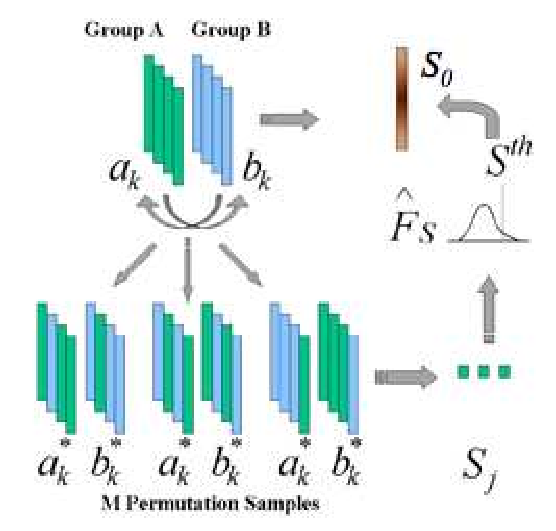
\includegraphics[width=6cm]{IJ_PermTests} &
      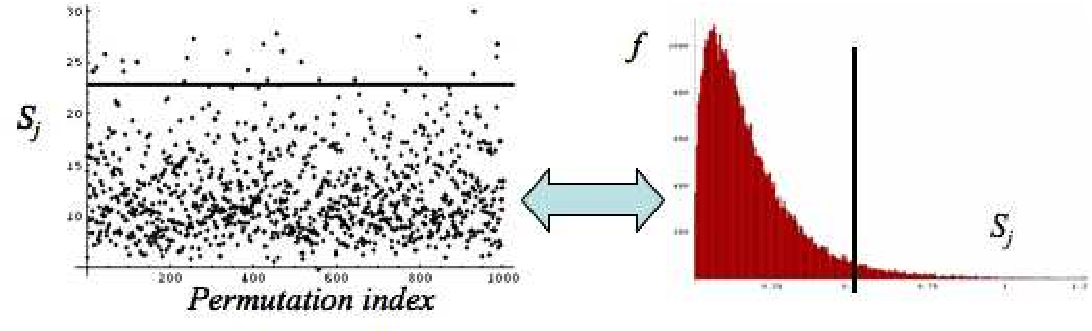
\includegraphics[width=9cm]{IJ_PermTests2} 
    \end{tabular}
    \itkcaption{Left: Scheme of P-value computation via permutation tests. The real group difference $S_0$ (e.g. Hotelling $T^2$) is compared to that the group differences  $S_j$ of random permutations of the group labels. The quantile in the $S_j$ histogram associated with $S_0$ is the p-value. Right: Example run on test data with 1000 random permutations. On the left the individual $S_j$ are plotted and on the left the corresponding $S_j$ histogram is shown. The black line indicates the value of $S_0$.}
   \label{fig:TestingPerm}
 \end{center}
\end{figure}

The significance of the mean difference metric (univariate: Student t, multivariate: Hotelling $T^2$) was next evaluate at each spatial location via a permutation test approach. Permutation
tests are a valid and tractable approach for such an application, as they rely on minimal assumptions and can be applied even when the assumptions of the parametric approach are untenable. Non-parametric permutation tests are exact, distribution free and adaptive to underlying correlation patterns in the data. Further, they are conceptually straightforward and, with recent
improvements in computing power, are computationally tractable. 

The null hypothesis is that the distribution of the locations
at each spatial element is the same for every subject regardless
of the group. Permutations among the two groups satisfy the exchangeability
condition, i.e. they leave the distribution of the statistic of interest
unaltered under the null hypothesis. Given $n_1$ members of the first group
$a_k$, $k=1 \ldots n_1$ and $n_2$ members of the second group $b_k$, $k=1
\ldots n_2$, we can create $M\leq $ \scriptsize $\left( \hspace{-0.1in}
\begin{tabular}{c}
$n_1+n_2$\\
$n_2$
\end{tabular}
\hspace{-0.1in} \right)$ \normalsize permutation samples. A value of M from
$20000$ and up should yield results that are negligibly different from using
all permutations \cite{edgington1995}.


\subsection{Correction for Multiple Comparison}

The local shape analysis involves testing from a few to many thousands of
hypothesis (one per surface element) for statistically significant effects.
It is thus important to control for the multiple testing problem, and the most
common measure of multiple false positives is the familywise error rate
(FWER). The multiple testing problem has been an active area of research in the
functional neuroimaging community. The most widely used methods in the
analysis of neuroimaging data use random field theory \cite{chung2001}
\cite{worsley1996} and make inferences based on the maximum distribution. In
this framework, a closed form approximation for the tail of the maximum
distribution is available, based on the expected value of the Euler
characteristic of the thresholded image \cite{worsley1996}. However, random
field theory relies on many assumptions such as the same parametric
distribution at each spatial location, a point spread function with two
derivatives at the origin, sufficient smoothness to justify the application
of the continuous random field theory, and a sufficiently high threshold for
the asymptotic results to be accurate.

In our work, we are employing non-parametric permutation tests and false discovery rate as two alternative correction methods for the multiple comparison problem.

\subsubsection{Minimum over Non-parametric permutation tests}

Non-parametric methods deal with the multiple comparisons problem \cite{PantazisISBI04}  and 
can be applied when the assumptions of the parametric approach are untenable.  Similar methods have
been applied in a wide range of functional imaging applications
\cite{Nichols2001,pantazis2003,sowell1999}. 

Details of this method are described in \cite{PantazisISBI04} and only a summary is provided here. The correction method is based on computing first the local p-values using permutation tests. The minimum of these p-values across the surface is then computed for every permutation (see Figure \ref{fig:TestingPerm} left). The appropriate corrected p-value at level $\alpha$ can then be obtained by computing the value at the $\alpha$-quantile in the histogram of these minimum values. Using the minimum statistic of the p-values, this method correctly controls for the FWER, or the false positives, but no control of the false negatives is provided. The resulting corrected local significance values can thus be regarded as pessimistic estimates akin to a simple Bonferroni correction.

\subsubsection{False Discovery Rate}

Additionally to the non-parametric permutation correction, a False Discovery Rate Estimation (FDR) \cite{FDR1995,FDR2002} method was also implemented and applied. This procedure controls the expected proportion of false positives only among those tests for which a local significance has been detected. The FDR method thus allows an expected proportion (usually 5\%) of the FDR corrected significance values to be falsely positive. The correction using FDR provides an interpretable and adaptive criterion with higher power than the non-parametric permutation tests. FDR is further simple to implement and computationally efficient even for large datasets.

The FDR correction (see Figure \ref{fig:TestingPerm} right) was computed as follows \cite{FDR2002}:
\begin{enumerate}
\item Select the desired FDR bound $q$, e.g. 5\%. This is the maximum proportion of false positives among the significant tests that you are willing to tolerate (on average).
\item Sort the p-values smallest to largest.
\item Let $p_q$ be the $p$-value for the largest index $i$ of the sorted p-values $p_{sort,i} \leq q \cdot i / N$, where N is the number of vertices.
\item Declare all locations with a p-value $p \leq p_q$ significant.
\end{enumerate}

\section{Methods}
\label{sec:meth}

The statistical framework proposed in this document differs from the traditional statistical analysis approach (see Figure \ref{fig:tradflow}) mainly in the inclusion of a step that consists in computing a General Linear Model (GLM) to test group differences at every surface location. The steps performed in this new proposed approach are shown in figure \ref{fig:newflow}.

\begin{figure}[htbp]
  \begin{center}
    \begin{tabular}[htbp]{c}
    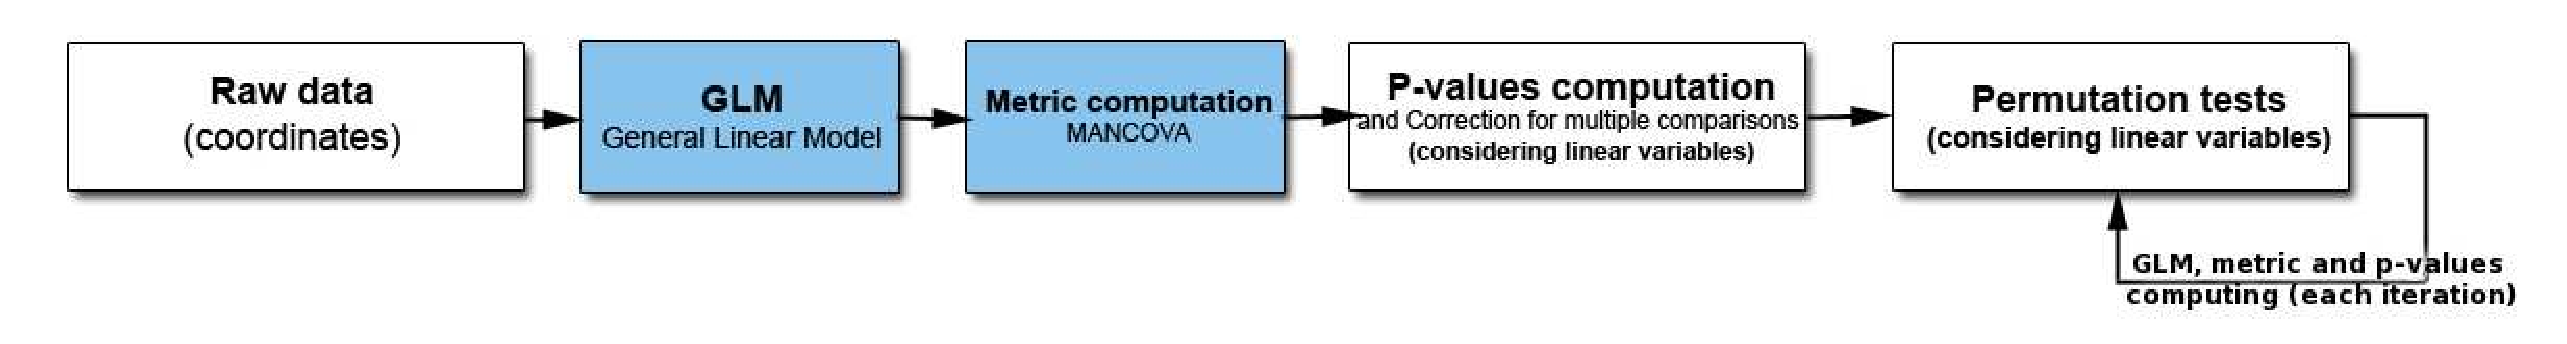
\includegraphics[width=0.9\textwidth]{IJ_NewAp}
    \end{tabular}
    \itkcaption{Workflow used for statistical analysis.}
    \label{fig:newflow}
  \end{center}
\end{figure}

In the following sections each one of these steps will be seen in detail. Some examples will be used in order to clarify the text.

\subsection{Linear Model}
\label{sec:linearmodel}

The main innovation in the new approach proposed is that we use a GLM to fit the observed raw data as follows:
\begin{equation}
Y = XB + U
\label{eq:GLM}
\end{equation}

Where $Y$ (nxd) is the observation matrix, $X$ (nxp) the design matrix, $B$ (pxd) is the parameter matrix and $U$ (nxd) the errormatrix. n = number of subjects, d = dimensionality of features, p = depends on design matrix. B is unknown, $X$ and $Y$ are known.

The parameter matrix B can be computing by solving the equation system as:
\begin{equation}
\hat{B} = (XX^T )^- \, X^TY ; (pxd)
\end{equation}

Where $X^-$ represents the pseudoinverse of the matrix.

Once parameter matrix B is known, the residual information after applying the GLM to the data is estimated as:
\begin{equation}
 E = (Y - X \hat{B})^T (Y - X \hat{B} ); (pxp)
\end{equation}  

This residual matrix E indicates the main eigenvalues of the data represented in the GLM.

\textbf{ EXAMPLE:} A case of study in which it is necessary to analyze shape changes of the caudate nucleii in an autistic population compared with a normal population, the observation matrix $Y$ contains row-wise the location vector $(x,y,z)$ (d = 3) for each subject both autistic and controls. $X$, the design matrix, contains the information of each subject variable. Nominal subject variables such as gender and diagnosis group are encoded as a set of binary, mutually exclusive variables. In case of considering gender, this would lead to a 4 binary variable $b_0$ contains 1 if the subject is male and control, and 0 otherwise, $b_1$ contains 1 if the subject is female and control and 0 otherwise, $b_2$ contains 1 if the subject is male and autistic patient and 0 otherwise, $b_3$ contains 1 if the subject is female and autistic patient and 0 otherwise.

\begin{center}
$Y = \left[ \begin{array}{cccc} x_1 & y_1 & z_1 \\ & \cdots & \\ x_n & y_n & z_n  \end{array} \right]$
\end{center}
\vspace{.1 in}


\begin{center}
$X = \left[ \begin{array}{ccccccc} b^1_0 & b^1_1 & b^1_2 & b^1_3 & age^1 & IQ^1 & score^1 \\ & & & \cdots & & & \\ b^n_0 & b^n_1 & b^n_2 & b^n_3 & age^n & IQ^n & score^n  \end{array} \right]$
\end{center}
\vspace{.1 in}

$\hat{B}$ will contain the estimates for the contributions relative to gender $\mu_i$, age $g$, IQ $q$ and scores $c$. All of these estimates are d-dimensional (3 in this example).
\vspace{.1 in}

\begin{center}
$\hat{B} = \left[ \begin{array}{ccc} \mu^x_0 & \mu^y_0 & \mu^z_0 \\ \mu^x_1 & \mu^y_1 & \mu^z_1 \\ \mu^x_2 & \mu^y_2 & \mu^z_2 \\ \mu^x_3 & \mu^y_3 & \mu^z_3 \\ g^x_1 & g^y_1 & g^z_1 \\ q^x_1 & q^y_1 & q^z_1 \\ c^x_1 & c^y_1 & c^z_1 \\   \end{array} \right]$
\end{center}


\subsection{Statistics}
\label{sec:stats}

Two matrices $A$ and $C$ are designed to capture the null hypothesis,  satisfying the relation:

\begin{equation}
\label{eq:ABC}
AB = C
\end{equation}

In the example, using the $B$ matrix given in section \ref{sec:linearmodel}, the null hypothesis to test would be that there is no difference between female autistic subjects and female normal controls and there is no difference between the male autistic subjects and the male normal controls. This hypothesis would be formulated with:

\vspace{.1 in}

\begin{center}
$A = \left[ \begin{array}{ccccccc} 1 & 0 & -1 & 0 & 0 & 0 & 0 \\ 0 & 1 & 0 & -1 & 0 & 0 & 0   \end{array} \right]$
\end{center}
\vspace{.1 in}

\begin{center}
$C = \left[ \begin{array}{ccc}  0 & 0 & 0 \\ 0 & 0 & 0   \end{array} \right]$
\end{center}
\vspace{.1 in}

%Added for Marc's comments:
The embedding of the null hypothesis into the matrices as described in equation (\ref{eq:ABC}) is very simple. When the multiplication $AB$ is made, 
it computes the difference between the average coordinates of the normal control and the autistic subjects. The top row is for males and the bottom row is for females. By having $C = 0$ , we are hypothesizing that there is no difference between the two groups or: $H_0 : \mu_{NC} = \mu_{Autistic}$ .

Having the remainder of the $A$ matrix as zeros allows for these variables to be `corrected for'. This is accomplished because by including these variables in the linear model that calculates $B$, their affect is modulated out, leaving a more accurate estimate of the average location of the points. We then formulate the null hypothesis with only these locations (the shape), and not the other factors that we are not currently evaluating.

In order to compute significance, we first calculate the MANCOVA hypothesis matrix:

\begin{equation}
H = (A\hat{B} - C)^T [A (X^TX)^- A^T]^{-1} (A\hat{B} - C)
\end{equation}

We now compute the three eigenvalues $\lambda_i$ of $H E^{-1}$ and we are given a choice of the following tests on these eigenvalues from \cite{Schlittgen09}:

\begin{eqnarray}
Wilks: \Lambda = \Pi(1 + \lambda_i)^{-1} \\
Hotelling: T^2_g =(n - r)\sum \lambda_i \\
Pillai : V^{(s)} = \sum \frac {\lambda_i} {1+ \lambda_i} \\
Roy : \lambda_{max} =max(\lambda_i)
\label{eq:stats}
\end{eqnarray}

For Wilks $\Lambda$ we employ a left-sided permutation test (min) in order to compute the p-value, whereas for Hotelling’s $T^2_g$, Pillai’s $V^{(s)}$ and Roy’s $\lambda_{max}$ we compute a right-sided permutation test (max) for the p-value. Any of these statistics can be used in the analysis by specifying the associated arguments.

\section{Program contents}
\label{sec:program}
The novel tool developed, \ProgramName, uses CMake \cite{CMake} as its cross-platform builder. This allows build scripts such as makefiles or project files to be customized to the specific machine.

In order to compile \ProgramName, ITK, VTK, GenerateCLP and Boost Libraries for C (v 0.39.1) must already be installed. CMake will ask for the directory where the aforementioned library files are located before creating the build scripts. 

\subsection{Input}
\label{sec:inputs}

The input arguments to the program are mainly for controlling the testing and output preferences, and to point to the data to be analyzed. The input file name is input in the first place in the command line and it will contain the list of mesh files that we want to analyze, as well as scale factors, categorical and associated variables. Combining the arguments input to the program and the information contained in the input file, two main tests can be performed:

\begin{itemize}
	\item \textit{Group Tests} If a simple group difference test is desired, it is necessary to specify the group being tested. By default it is the first group defined in the data input file, but you can choose which group to test by specifying the right argument (`--testColumn 1'). The default significance level for the p-values computing is 0.05, but any other value can be given on the command line as `--significanceLevel 0.01'. The number of permutations allowed in the statistical significance computing can be also changed. The default value of 10,000 is heuristically sufficient. More advanced analysis of the confidence interval for the p-value can be found in \cite{Seber04}. This value can be set higher (for higher confidence in the results) or lower (for increased speed) with the argument `--numPerms 5000'. 
	\item \textit{Interaction Tests}  If corrected statistics using independent variable(s) are desired, it will be also necessary to specify the variable tested. In \ref{fig:input}, the independent variable given is the age of the child at the time of the scan. The program will ignore this data unless the argument relative to independent variables is specified. When specifying the proper argument, the program performs the Interaction Tests that will correct the statistics computed using the specified independent variables. That is to say, \ProgramName correlates any independent variable with the shape at each point when performing the statistical computing. This is done with the permutation test methods described in \ref{sec:intro}. Spearman and Pearson correlation coefficients are also calculated if needed, testing the correlation of the independent variable with the shape changes. These shape changes will be quantified in two different ways: first by the length of the mean difference vector at each location and the projection of that vector onto the outward pointing normal on the mean surface. Both of these values are signed positive or negative depending on the direction of the vector of the mean difference vector compared to the surface normal vector.
\end{itemize}

Both input arguments and input file will be described in detail in the next sections. 

\subsubsection{Input file}
\label{sec:ifile} 

Following the example used in section \ref{sec:linearmodel} an input file can be composed to perform the statistical analysis. In Figure \ref{fig:input}, the first column contains a 0 for autistic or a 4 for normal control (diagnostic group type). In the same way, the second column offers information regarding to gender group type. This is additional data that will set up two groups, diagnostic group and gender group, and it needs to be specified (`--numGroupTypes 2' argument). Depending on the number of group types N, the system will compute all combinations among them i.e. $2^N$ combinations. The third column in figure \ref{fig:input} contains the scale factor for each mesh file. Each point in the mesh associated with this subject will be scaled by this amount, but only if the correspondent command line argument is also present (`--scale'). The next column is an absolute or relative path to the mesh file. An error will be generated if the file does not contain a mesh or does not exist. The last column (or columns) contains data regarding to the linear variables associated with the mesh. This data will be used in the creation of the GLM and in case of performing Interaction Tests. 

\begin{figure}[htbp]
  \begin{center}
    \begin{tabular}[htbp]{c}
    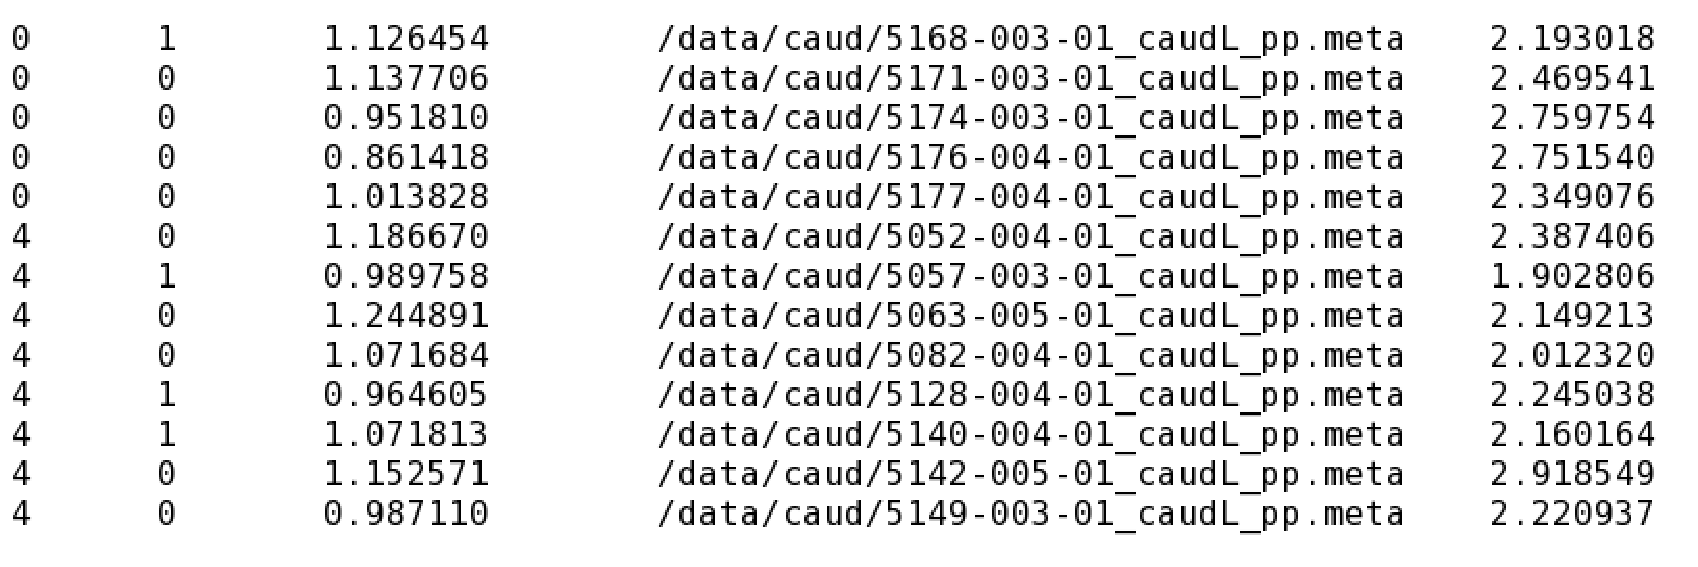
\includegraphics[width=0.8\textwidth]{IJ_InputFile}
    \end{tabular}
   \itkcaption{A screenshot of an example mesh-list input file.}
   \label{fig:input}
  \end{center}
\end{figure}

\subsubsection{Input arguments}
\label{sec:iargs} 

\ProgramName offers different statistical functionalities that can allow the user to perform and design a statistical analysis. The input arguments allow to tune the program in order to obtain the desired results.

\begin{itemize}
	\item \texttt{\textbf{\small {`<std::string>'}}}  (required)  File which contains all of the data to be analyzed. File is a list pointing to other data sources.
	\item \texttt{\small {`--processinformationaddress <std::string>'}}  Address of a structure to store process information (progress, abort, etc.). (default: 0)
	\item \texttt{\small {`--xml'}}  Produce xml description of command line arguments (default: 0)
	\item \texttt{\small {`--echo'}}  Echo the command line arguments (default: 0)
	\item \texttt{\small {`--trendCorrelation'}}  For the simple (non-MANCOVA) correlation, test for correlation. (default: 0)
	\item \texttt{\small {`--positiveCorrelation'}}  For the simple (non-MANCOVA) correlation, test for positive correlation.(Only works in conjunction with parametric testing!)     (default: 0)
	\item \texttt{\small {`--negativeCorrelation'}}  For the simple (non-MANCOVA) correlation, test for negative correlation. (Only works in conjunction with parametric testing!)      (default: 0)
	\item \texttt{\small {`--pillai'}}  Uses Pillai statistic for MANCOVA testing. (default: 0)
   	\item \texttt{\small {`--hotelling'}}  Uses Hotelling statistic for MANCOVA testing. (default: 0)
     	\item \texttt{\small {`--wilks'}}  Uses Wilks statistic for MANCOVA testing. (default: 0)
     	\item \texttt{\small {`--roy'}}  Uses Roy statistic for MANCOVA testing. (default: 0)
     	\item \texttt{\small {`--debug'}}  Outputs additional debugging information. (default: 0)
     	\item \texttt{\small {`--scale'}}  Scale all point data by the cube-root of the scale factor found in the input file. This is typically used for correcting differences such as      varying intercranial volumes (ICV). (default: 0)
     	\item \texttt{\small {`--simpleCorrsParaP'}}  Computes the p-value parametrically for the simple correlation test. (default: 0)
     	\item \texttt{\small {`--simpleCorrs'}}  Simple Spearman and Pearson correlations are computed, based on the normal to the average shape. This option is only valid in interaction test mode. (default: 0)
     	\item \texttt{\small {`--interactionTest'}}  Instead of a group test, simply test for statistically significant interaction of the data with a single independent variable. (default:
     0)
     	\item \texttt{\small {`--computeScaleFactorFromVolumes'}}  Reinterprets the scaling column values as volumes and compute the scaling factor from them. WARNING: This is different from the traditional file format where these scaling were already pre-computed. (default: 0)
     	\item \texttt{\small {`--writeZScores'}}  Writes out the z-scores. Only uses group assignments from the first group column currently. z-score of group A is computed with mean and standard deviation from group B and vice versa. z-scores are output based on the projections on the mean surface normal as well as the corresponding Mahalanobis distances (where no projection is performed). (default: 0)
     	\item \texttt{\small {`--significanceLevel <double>'}}  What cutoff of p-values is considered significant. Only affects the FDR corrected results. (default: 0.05)
     	\item \texttt{\small {`--testColumn <int>'}}   Which column of the data is being tested (0 based). If this is a standard 'Group Test', it will be one of the group columns. If it is an 'Interaction Test', it will be one of the independent variable columns. (default: 0)
      	\item \texttt{\small {`--numIndependent <int>'}}  Number of different independent variables associated with each subject. (default: 0)
     	\item \texttt{\small {`--numGroupTypes <int>'}}  Number of different classification types. (default: 1)
     	\item \texttt{\small {`--numPerms <int>'}}  Number of permutations to perform. (default: 10000)
     	\item \texttt{\small {`--out <std::string>'}}  All output files will have this as their base. (default: statResult)
	\item \texttt{\small {`--ignore\_rest'}}  Ignores the rest of the labeled arguments following this flag.
	\item \texttt{\small {`--version'}}  Displays version information and exits.
	\item \texttt{\small {`--help'}}  Displays usage information and exits.
\end{itemize}

\subsection{Output}
\label{sec:outputs}

\ProgramName outputs diverse files. The first type of output files are given as text files containing a header and a list of values associated with each point in the surface, those list of values can be one dimensional (scalar) or three-dimensional (vectors). The header contains the type of data, the dimensionality of data, and the number of points included. The second type of output files contain full shape data in form of mesh definitions. These are composed of a list of point locations, and then a list with full connectivity information for the triangles conecting each point. All these files all have a '*.meta' extension and are in ITK Spatial object mesh format. They can be easily visualized using \emph{KWMeshVisu} \cite{Oguz06} and 3D Slicer (v3.3 and above). Both types of files will be described next.

\subsubsection{Text files}
\label{sec:tfiles} 

\begin{itemize}
	\item `\_diffMesh.txt' includes the difference vectors obtained from the subtraction of two mean shapes from the groups tested.
	\item `\_normDistance.txt' includes the magnitude of the difference vectors. 
	\item `\_normProjections.txt' includes the magnitude of the projection of the previously described difference vectors to its correspondent normal vector in the mean population surface. The magnitude of this projection is a measure of shape variation that can be useful in the analysis.
	\item `\_mancovarawP.txt' includes the raw p-values or associated statistical significance for each point for the test performed. 
	\item `\_mancovaFDRP.txt' includes the p-values after correction for false discovery. False Discovery Rate (FDR) \cite{Genovese02} threshold is calculated first, and then the raw p-values are scaled considering that the FDR threshold is now at the given significance level.
	\item `\_mancovaBonferroniP.txt' includes the p-values after Bonferroni correction. Bonferroni correction (FDR) threshold is calculated first, and then the raw p-values are scaled considering that the Bonferroni threshold is now at the given significance level.
	\item `\_*Spearman.txt' includes a collection of files are generated when the right argument (`--simpleCorrs') is used in an Interaction Test. Those files will include raw P values maps, corrected FDR maps, Bonferroni corrected P values maps, and the Spearman correlation coefficients maps for a population of shapes correlated with a certain independent variable. The correlation is calculated for both normDistProjections shape scalar maps and normProjections shape scalar maps.
	\item `\_*Pearson.txt' includes a collection of files are generated correlation is used an Interaction Test. In the same way than the one described for Spearman correlation, the files will contain raw P values maps, corrected FDR maps, Bonferroni corrected P values maps, and the Pearson correlation coefficients maps for a population of shapes correlated with a certain independent variable. The correlation is calculated for both normDistances shape scalar maps and normProjections shape scalar maps. Both Pearson and Spearman correlation related files are always computed.
	\item `\_*localZ.txt' includes the Z-scores maps for a given population of shapes in a Group Test. This score is a dimensionless quantity derived for each point in a surface from group A by subtracting the group B mean from the individual raw shape score and then dividing the difference by the group B standard deviation. This score indicates how much each an individual in group A point varies from the composite model of all the surfaces in group B. For subjects in group B, this score is computed with respect to the composite model of all surfaces in group A.
\end{itemize}

\subsubsection{Mesh files}
\label{sec:mfiles} 

\begin{itemize}
	\item `\_meanAll\_uncorrected.meta' includes the overall population mean shape without GLM correction.
	\item `\_meanA.meta' and `\_meanB.meta' contain mean shape of each one of the two groups being tested.
	\item `\_GLM\_corrected\_meanAll.meta' is calculated only in case of Interaction Tests, and it contains the overall mean shape corrected using the values of the indicated independent variables. The General Linear Model (GLM) used in this correction follows equation (\ref{eq:GLM}).  
\end{itemize}

\section{Groupwise Analysis Scenarios}
\label{sec:results}
In order to further clarify the methods and to show  \ProgramName \textit{ } statistical power, three analysis scenarios are going to be exposed in the following sections. The first analysis scenario shows the results and conclusions obtained from a cross-sectional groupwise study. This scenario is the same one used as example in section \ref{sec:meth}. The second analysis scenario presents the results obtained in a longitudinal study, trying to capture special features of a certain disease progression in different subjects, that will be also compared in a groupwise fashion. Finally, a third analysis scenario will show the power of the tool to correlate shape variation groupwise features with clinical scores.

\subsection{Cross-sectional growpwise analysis scenario}
\label{sec:crosssec}

Data from 52 autistic and 22 typically developing children between 18 and 35 months (2 years) of age was studied to investigate shape changes associated with autism (see also \cite{Hazlett05}). The caudate nucleus in each brain scan were expertly segmented and preprocessed as discussed in \cite{Styner06}. 

\subsubsection{Hypothesis formulation}
\label{sec:hypho}


Depending on the hypothesis formulated for any specific group test, the permutation is performed on individual sets of parameters of the design matrix $X$. The necessary parameters for the Group Test design will be input in the final program as different arguments, that will be discussed in detail in section \ref{sec:inputs}. 

\vspace{.1 in}
\begin{center}
$X = \left[ \begin{array}{ccccccc} b^1_0 & b^1_1 & b^1_2 & b^1_3 & age^1 & IQ^1 & score^1 \\ & & & \cdots & & & \\ b^n_0 & b^n_1 & b^n_2 & b^n_3 & age^n & IQ^n & score^n  \end{array} \right]$
\end{center}
\vspace{.1 in}

Several hypothesis could be formulated in order to perform different Group Tests in this specific case:

\textbf{ Hypothesis 1:} Is there a significant difference between groups after correction for gender, age, IQ and clinical behavioral score? Permute binary variables of group identification (keeping the gender constant). Create a permutation that leads to switches of $b_0$ and $b_2$, as well as $b_1$ and $b_3$.

Example command: `\program infile - -numGroupTypes 2 - -numIndependent 3'

\textbf{Hypothesis 2:} Is there a significant age influence after correction for group, gender, IQ and clinical score? Simply permute the ’age’ parameter in $X$.

Example command: `\program infile - -numGroupTypes 2 - -numIndependent 3 - -interactionTest'

\textbf{Hypothesis 3:} Is there a significant clinical score influence after correction for group, gender, age and IQ? Simply permute the ’clinical score’ parameter in $X$.

Example command: `\program infile - -numGroupTypes 2 - -numIndependent 3 - -interactionTest - -testColumn 2'
%If changed to 1-based, should be 3

\subsubsection{Results}
\label{sec:lilresults}

All the color maps calculated will be displayed on the average surfaces of the mesh population. In case of performing a Group Test using the diagnostic group (autistic vs normal controls) the mean difference vectors are show in figure \ref{fig:meanA} and figure \ref{fig:meanDiff} (left). Those vectors show the differences in the morphology of the average surface of autistic caudate nucleii surfaces compared with the morphology of the average normal control surface. These mean difference vectors show clearly an overall bending action on the autistic average caudate, displaying vectors pointing away from the head and tail. 

The magnitude of the projection of these difference vectors onto the normals colour map is shown in \ref{fig:meanDiff} (right). This map shows shape group changes over the average surface. White color is used where there are no relevant changes (magnitudes equals zero). The color gets darker as the magnitudes of change increase. The distance is positive if the mean surface of the autistic population is protruding outside of the mean surface of normal controls; the distance is negative if the mean surface of autistic population is shrinking below the mean surface of normal controls. Positive distances are color-coded by blue and negative distances are color-coded by red.

Figure \ref{fig:rawP} (left) shows statistical significance for morphological changes. A color coded p-values map can be visualized over a mean surface. In the map, highly significant correlations ($p < 0.01$) are color-coded with red, intermediately significant correlations are color-coded with green ($0.01 > p > 0.05$) and non-significant correlations are color-coded with blue. The main area of significance for our case of study is located on the head of the caudate. This area of the caudate has been demonstrated to be highly involved in learning and memory and also associated with repetitive tasks performance.

Behavioral scores were used to perform Interaction Tests. Morphological changes analysis correlated with the overall behavioral score results are shown in figure \ref{fig:rawP} (right).

\begin{figure}[htbp]
  \begin{center}
    \begin{tabular}[htbp]{c}
    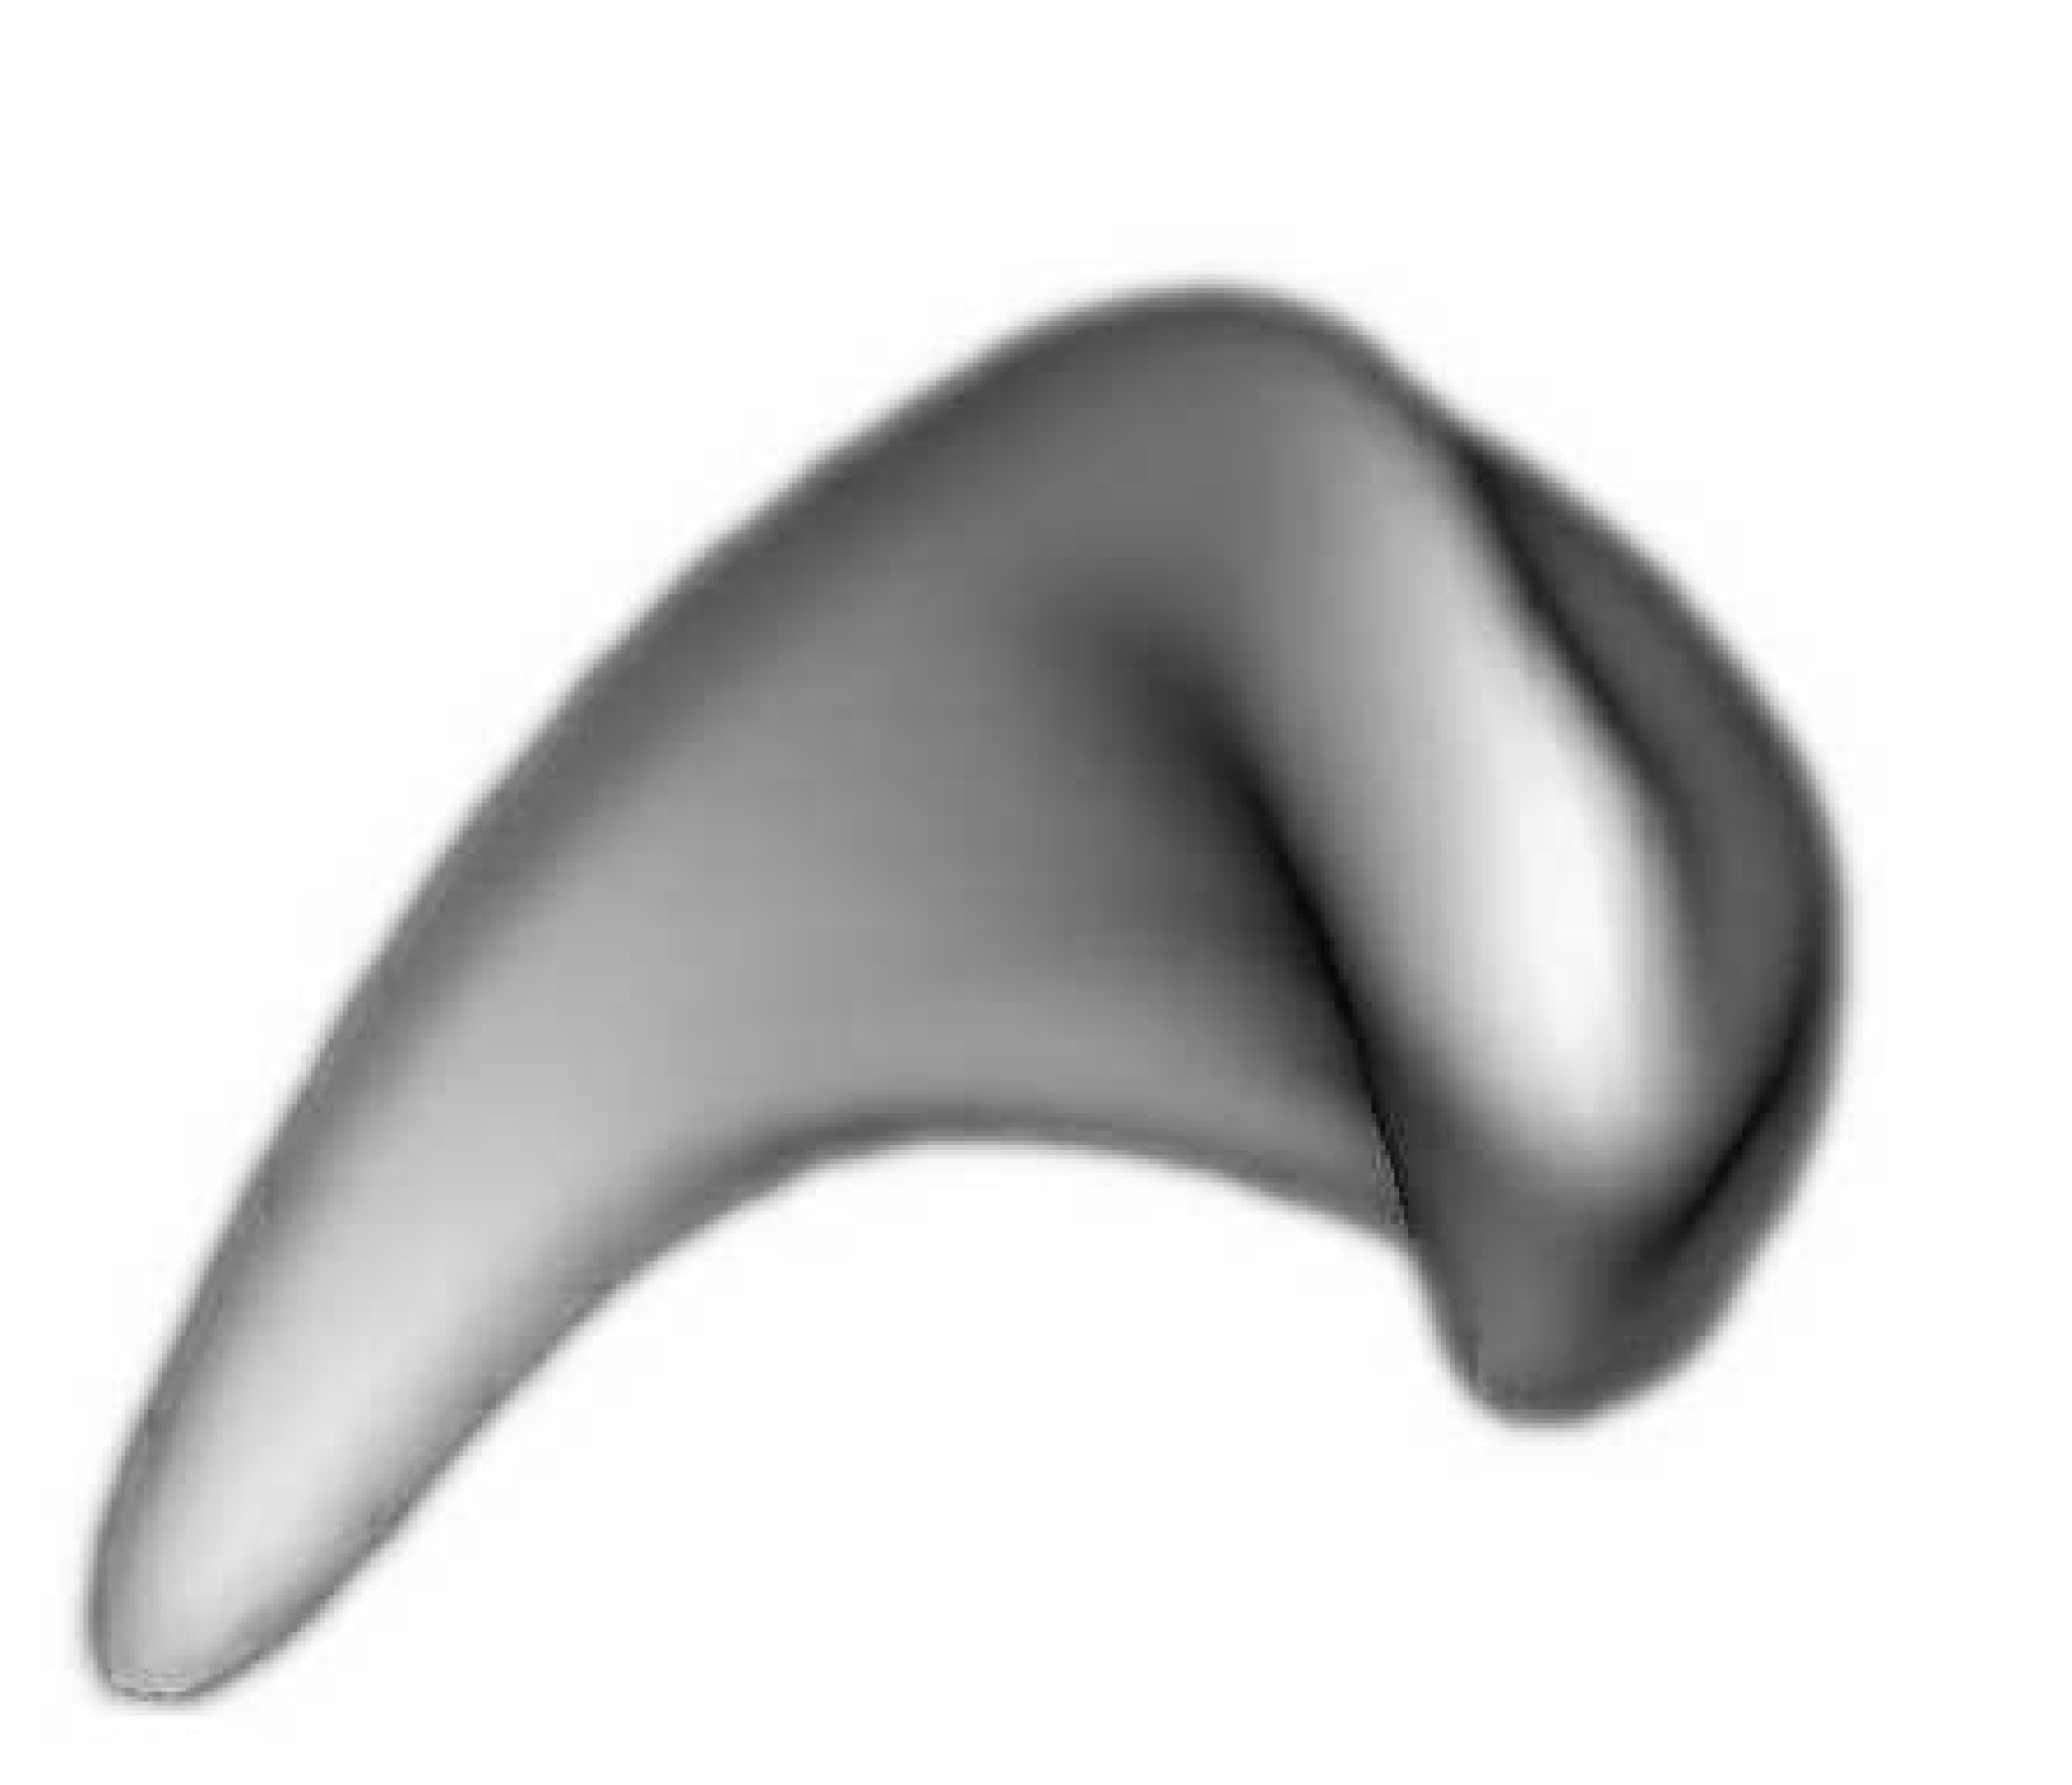
\includegraphics[width=6cm]{IJ_AnalysisScenario1_MeanA} 
    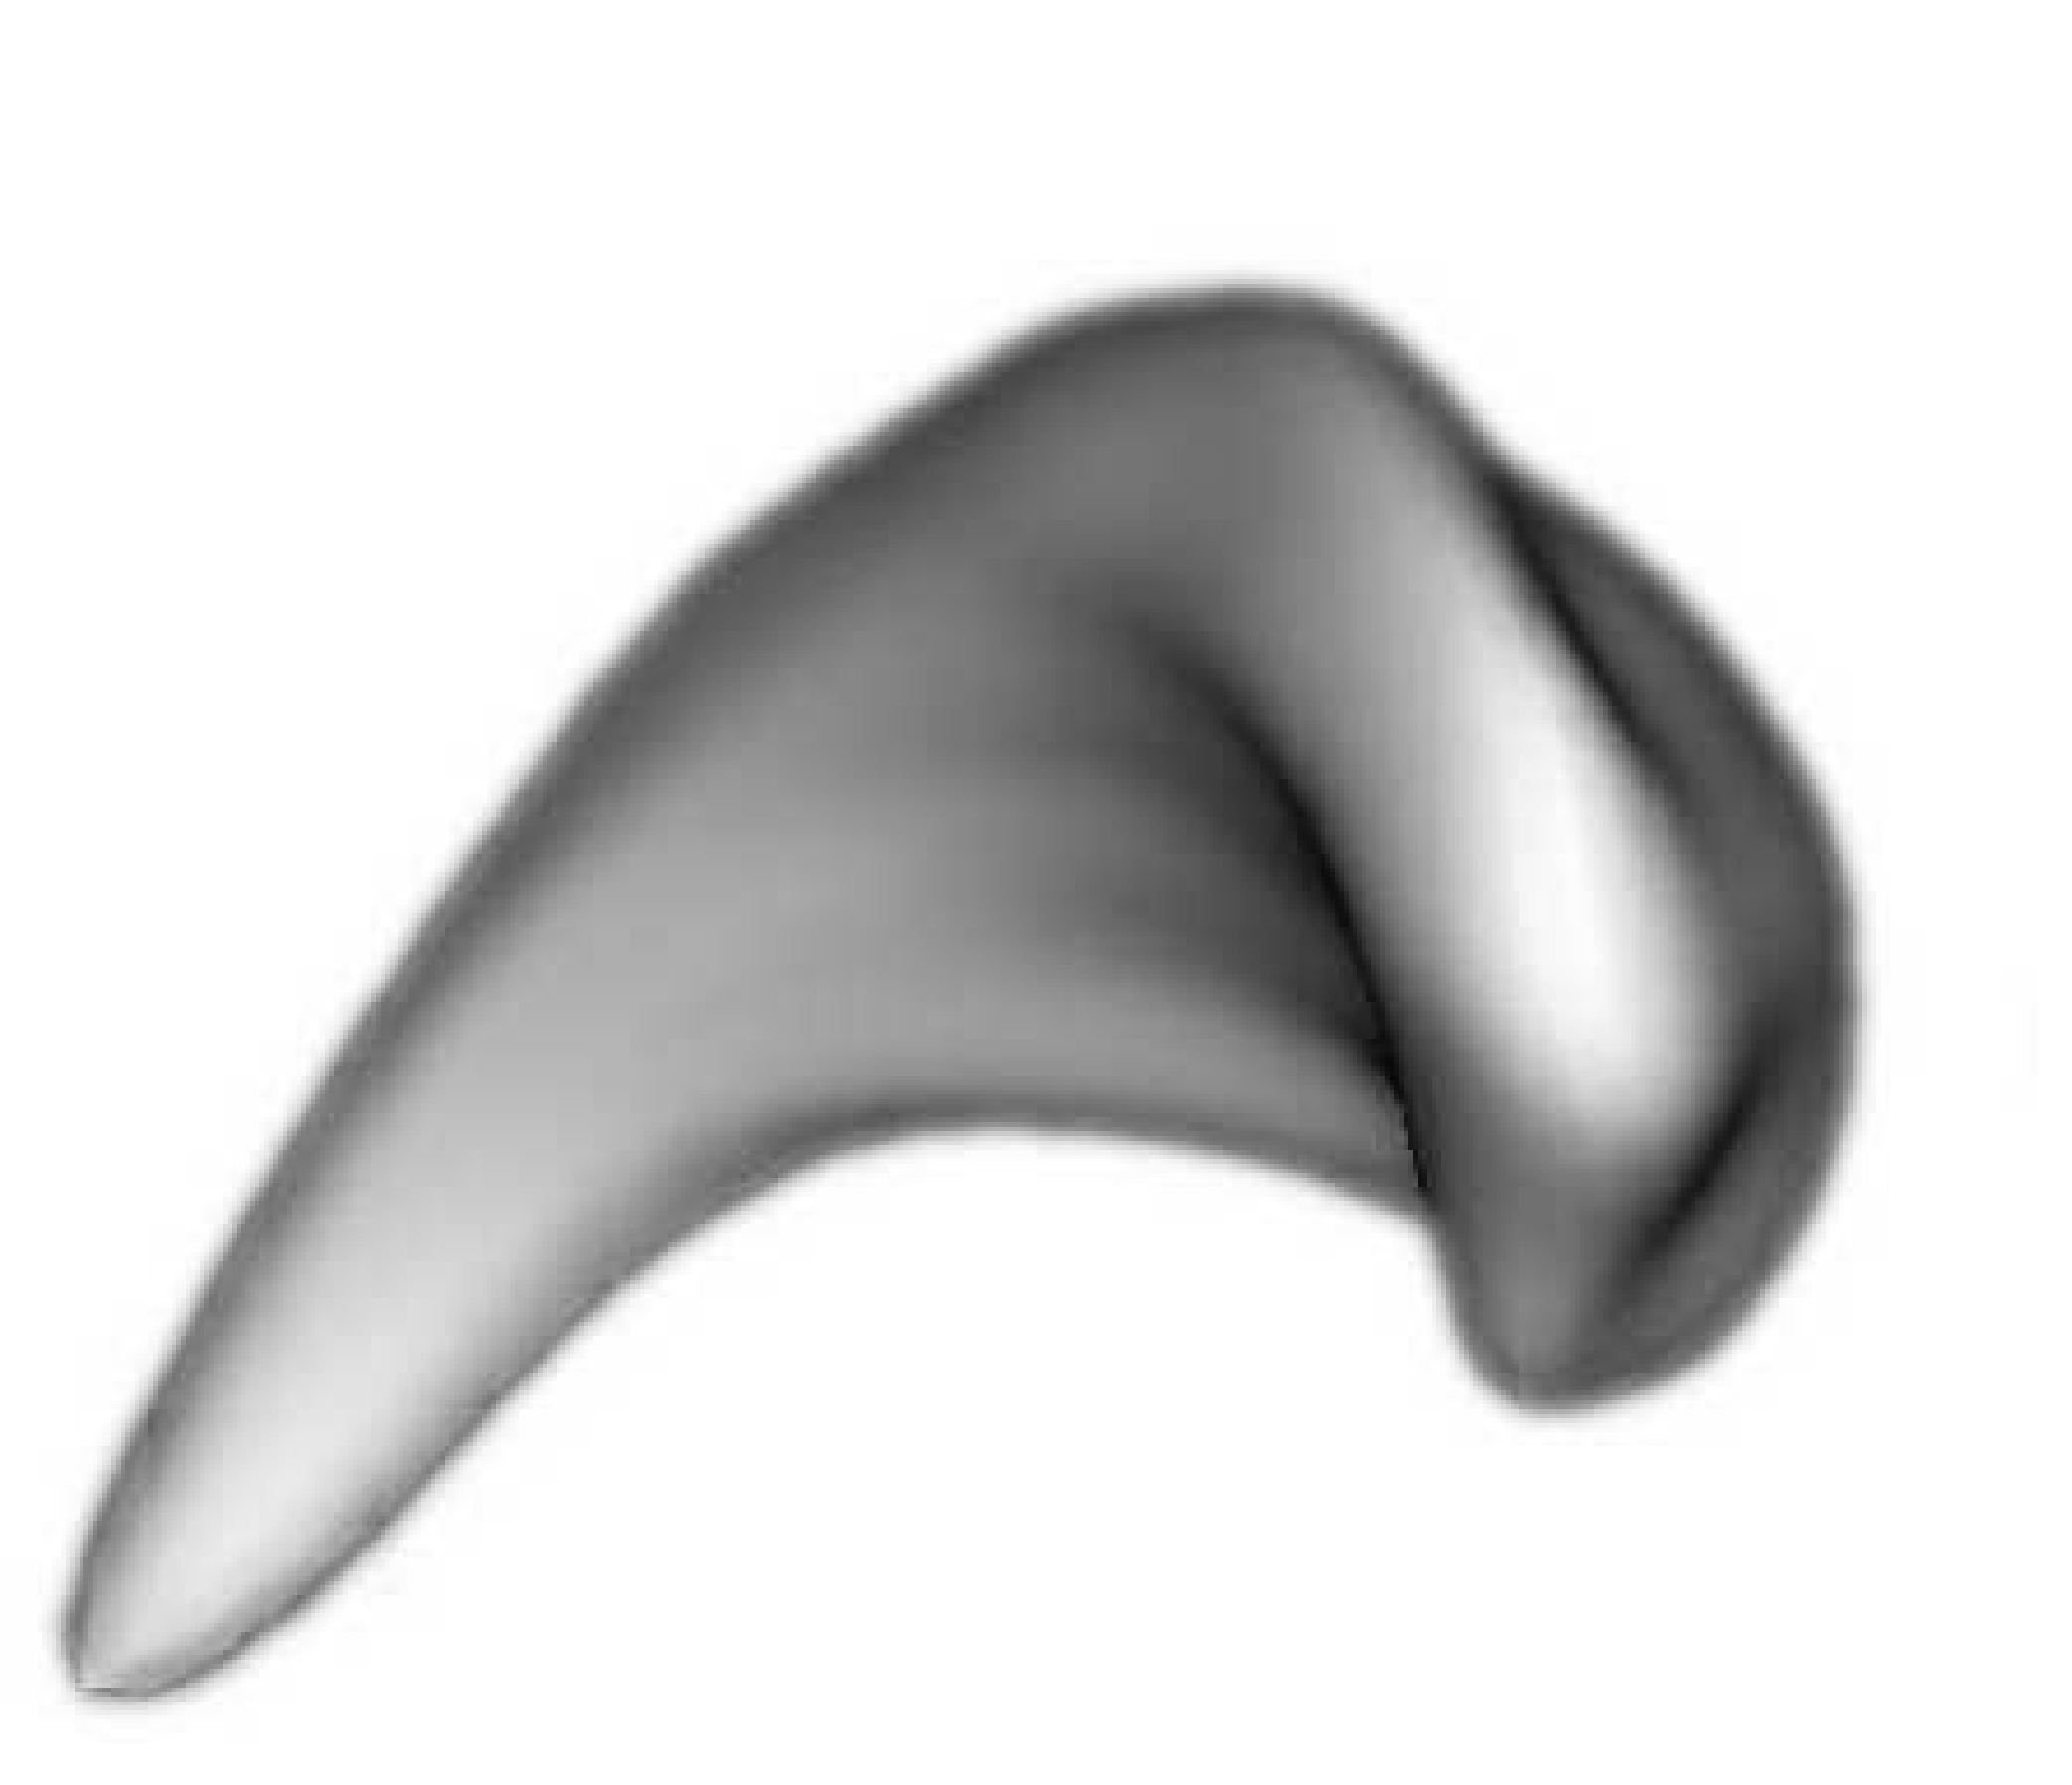
\includegraphics[width=6cm]{IJ_AnalysisScenario1_MeanB}
    \end{tabular}
    \itkcaption{Left: Mean shape of the caudate for the autistic population. Right: Mean shape of the caudate for the normal control (NC) population.}
    \label{fig:meanA}
  \end{center}
\end{figure}

\begin{figure}[htbp]
  \begin{center}
    \begin{tabular}[htbp]{c}
    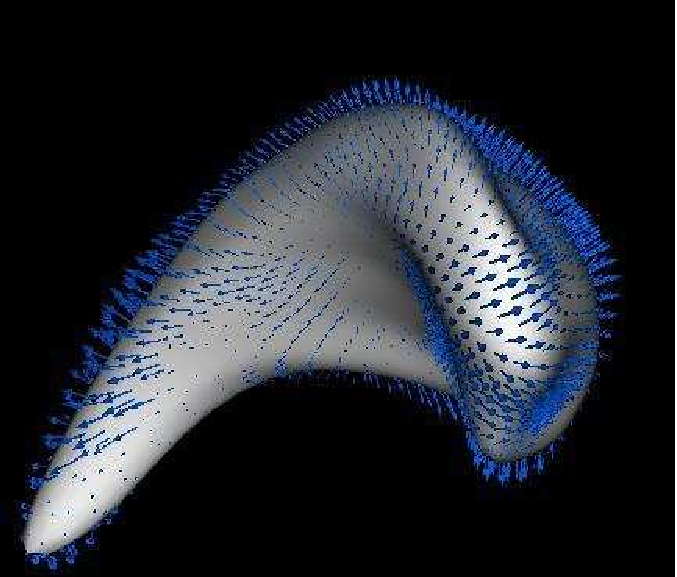
\includegraphics[width=6cm]{IJ_AnalysisScenario1_MeanDiff}
    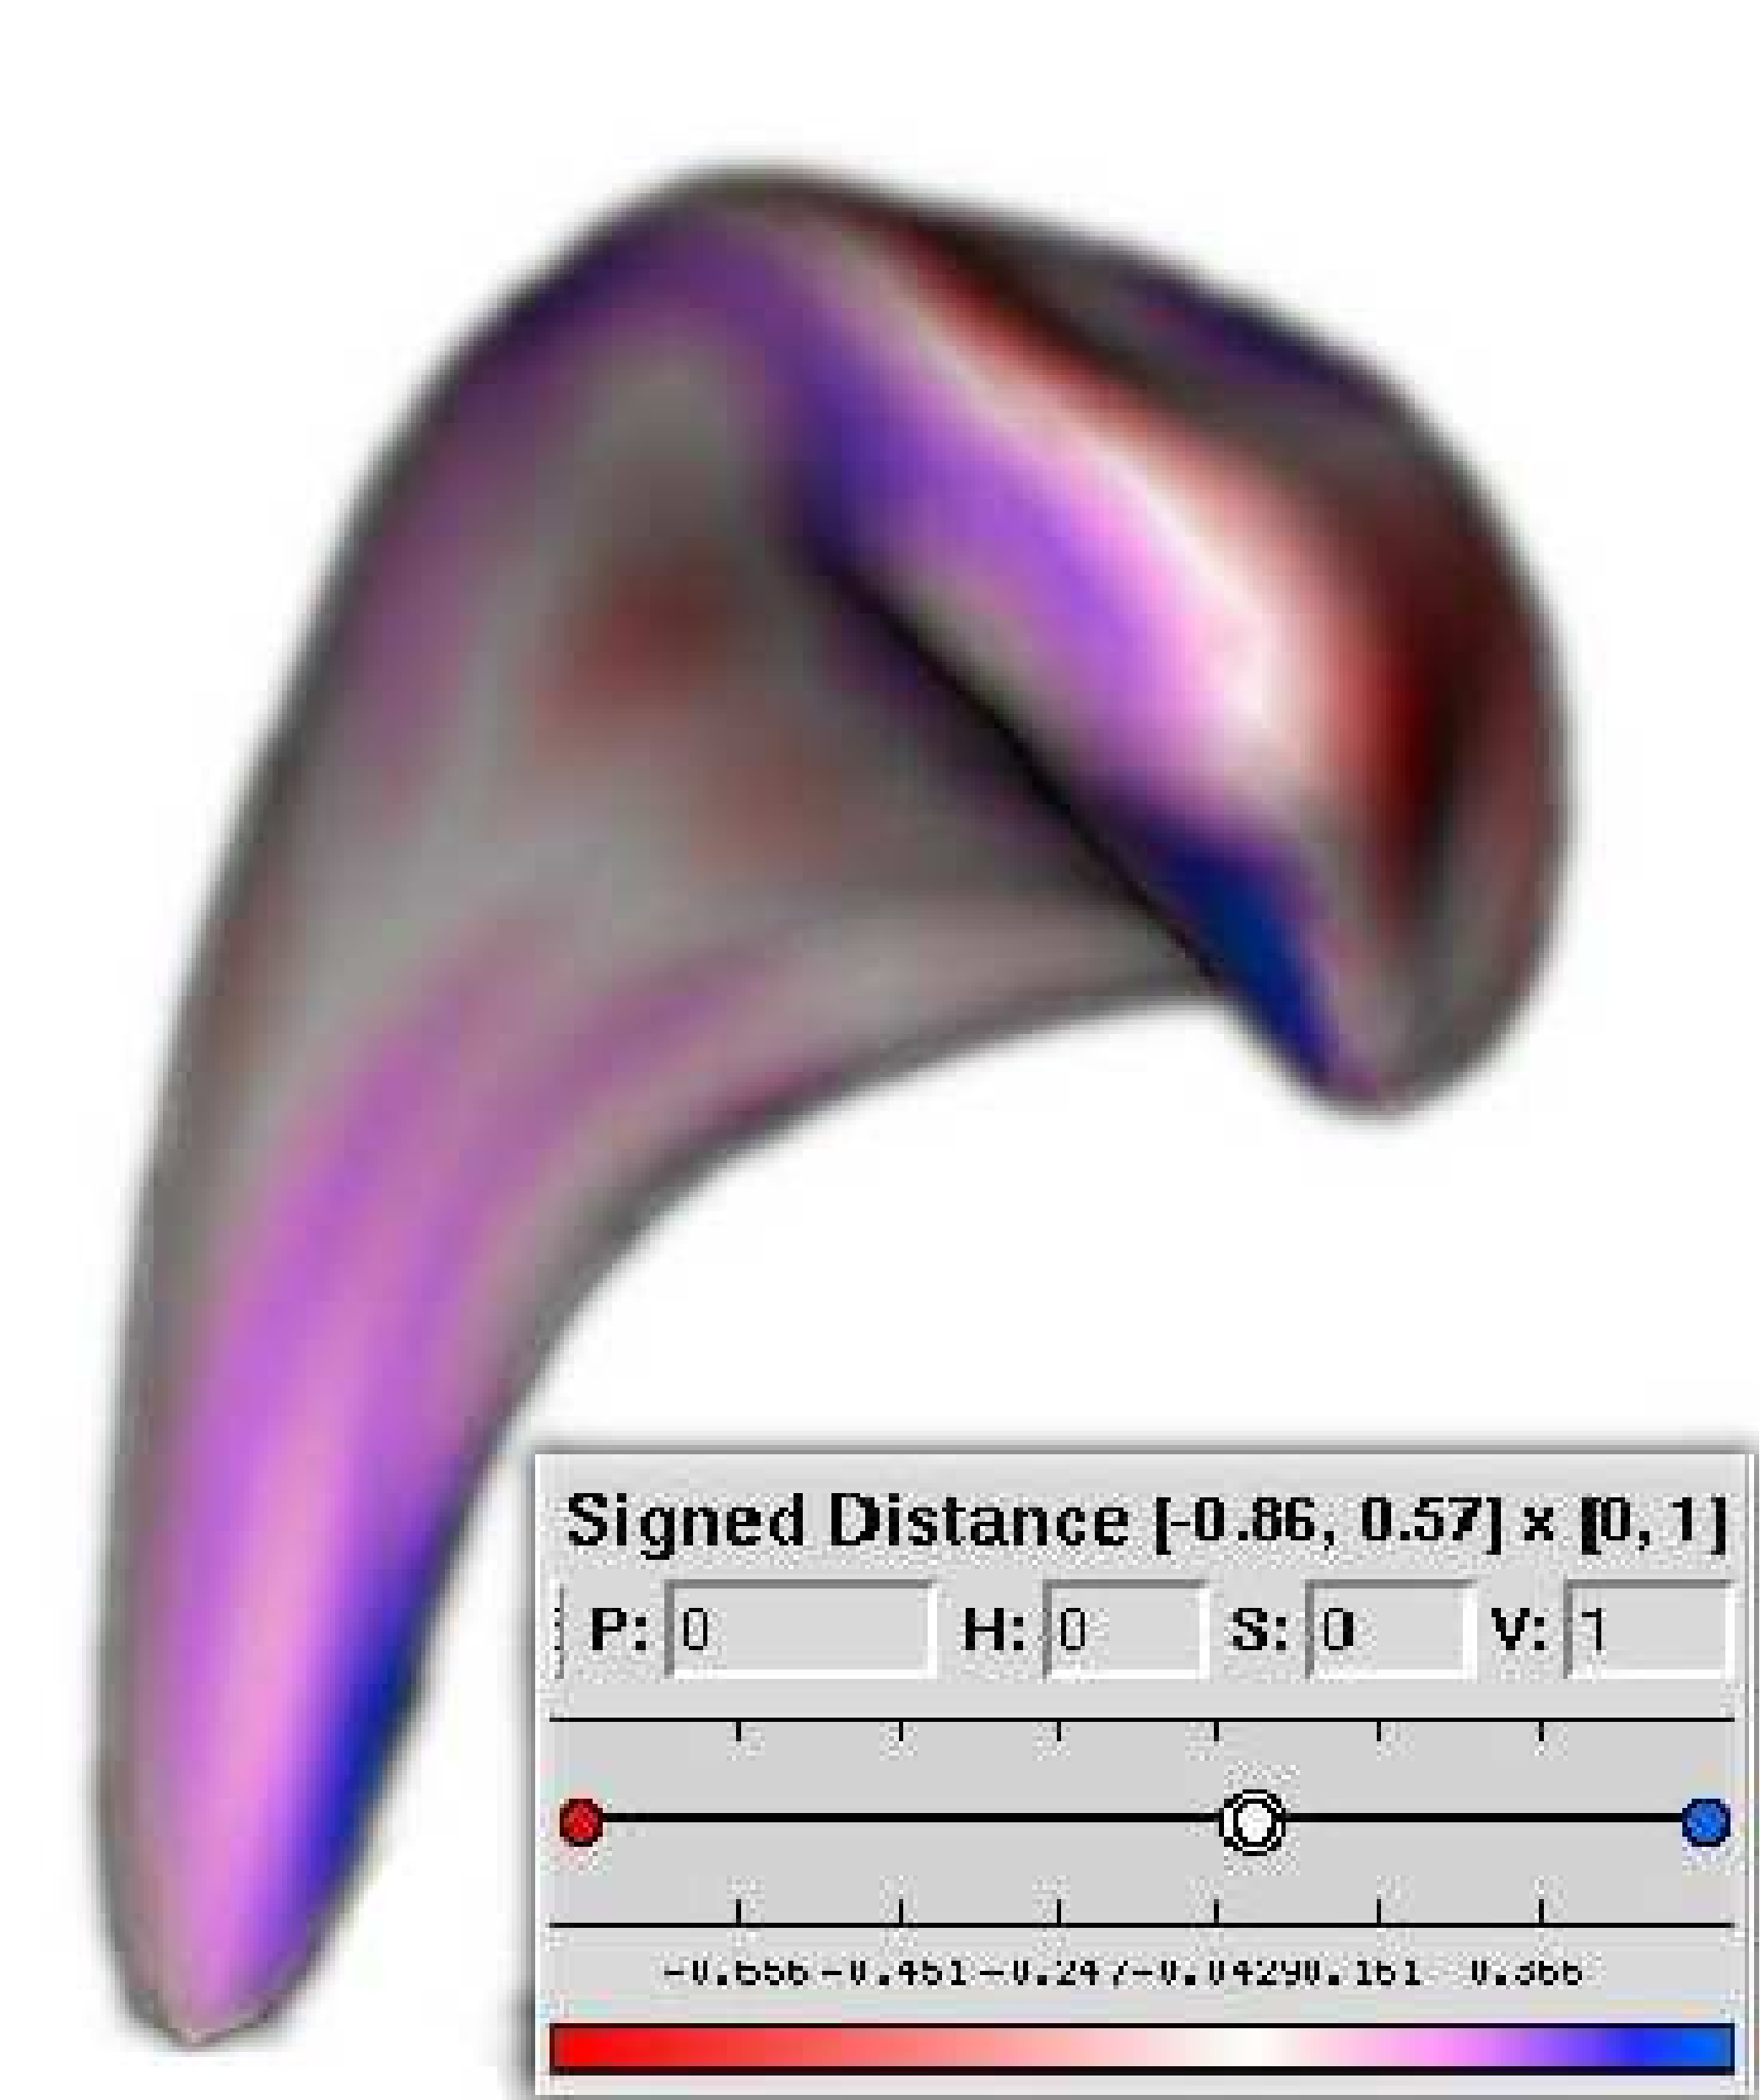
\includegraphics[width=6cm]{IJ_AnalysisScenario1_NormProjections}
    \end{tabular}
   \itkcaption{Left: Mean shape of the caudate for the NC population showing the vectors that point to the autistic mean shape. Right: The value of the mean difference vector projected onto the signed normal. Notice that the top of the head is moving negatively (into the shape) while the bottom of the head and the tail are moving positively (out of the shape). This seems to indicate a bending motion.}
    \label{fig:meanDiff}
  \end{center}
\end{figure}

\begin{figure}[htbp]
  \begin{center}
    \begin{tabular}[htbp]{c}
    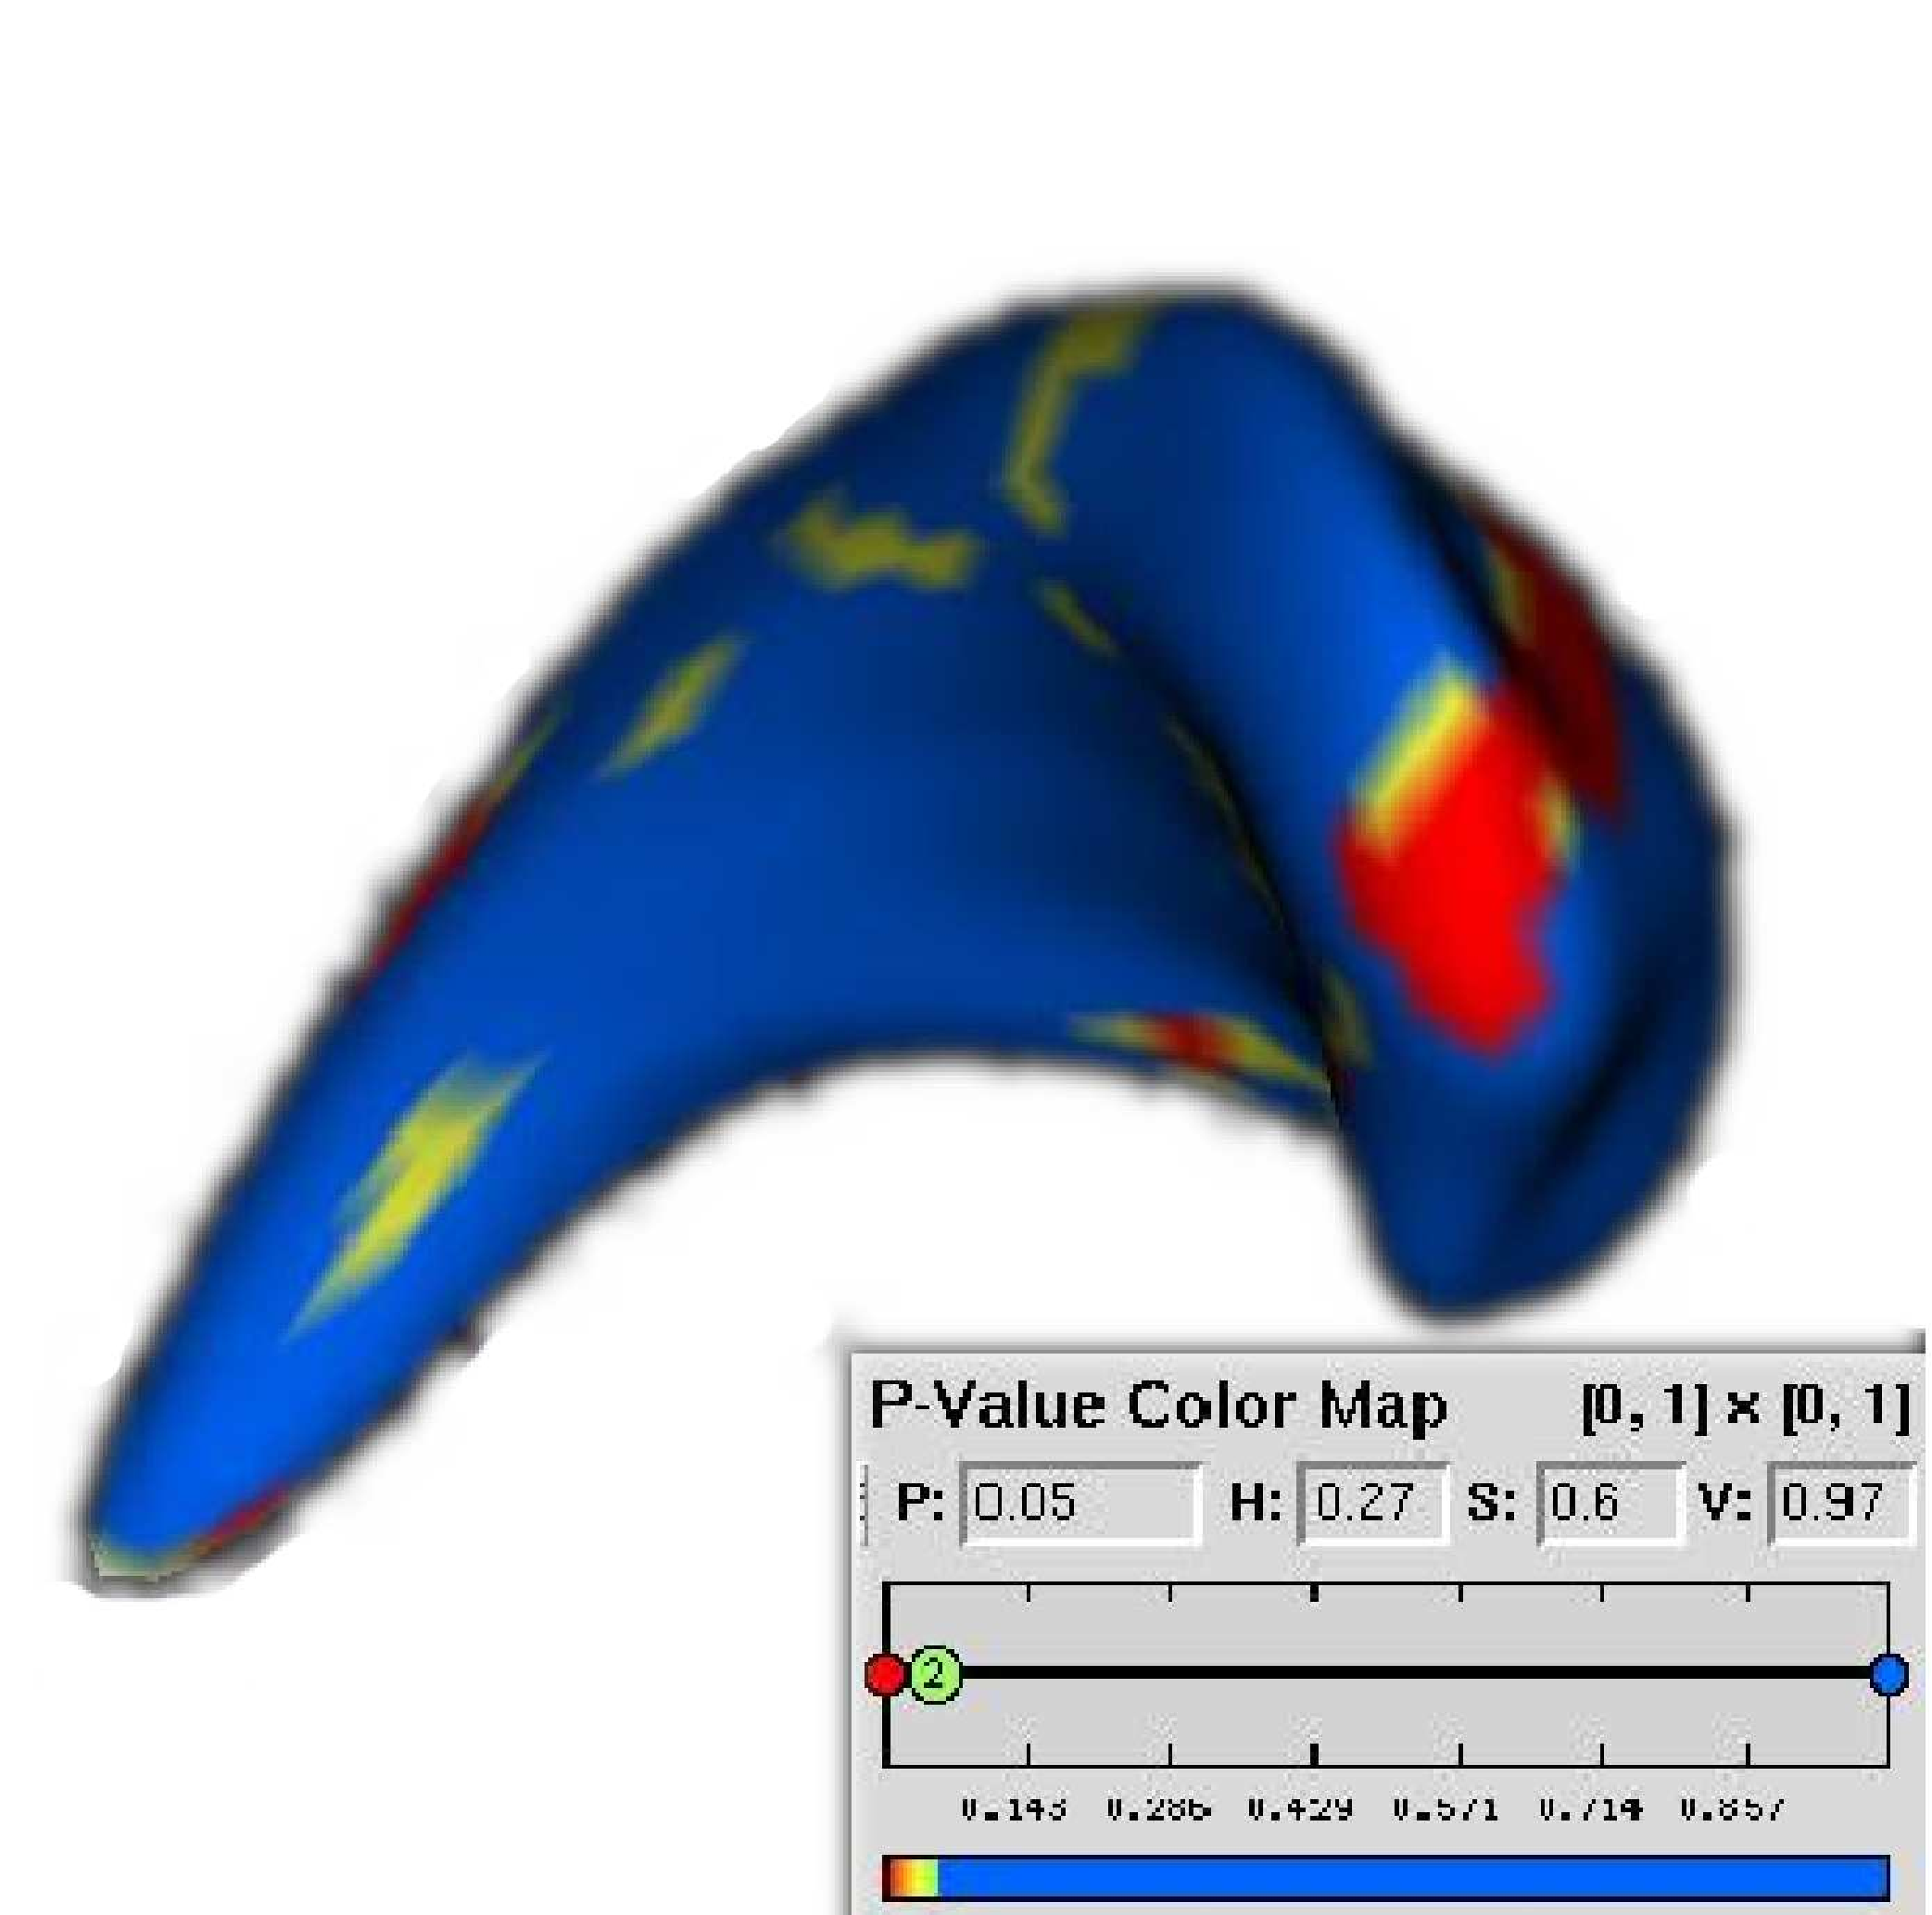
\includegraphics[width=6cm]{IJ_AnalysisScenario1_RawPValues}
    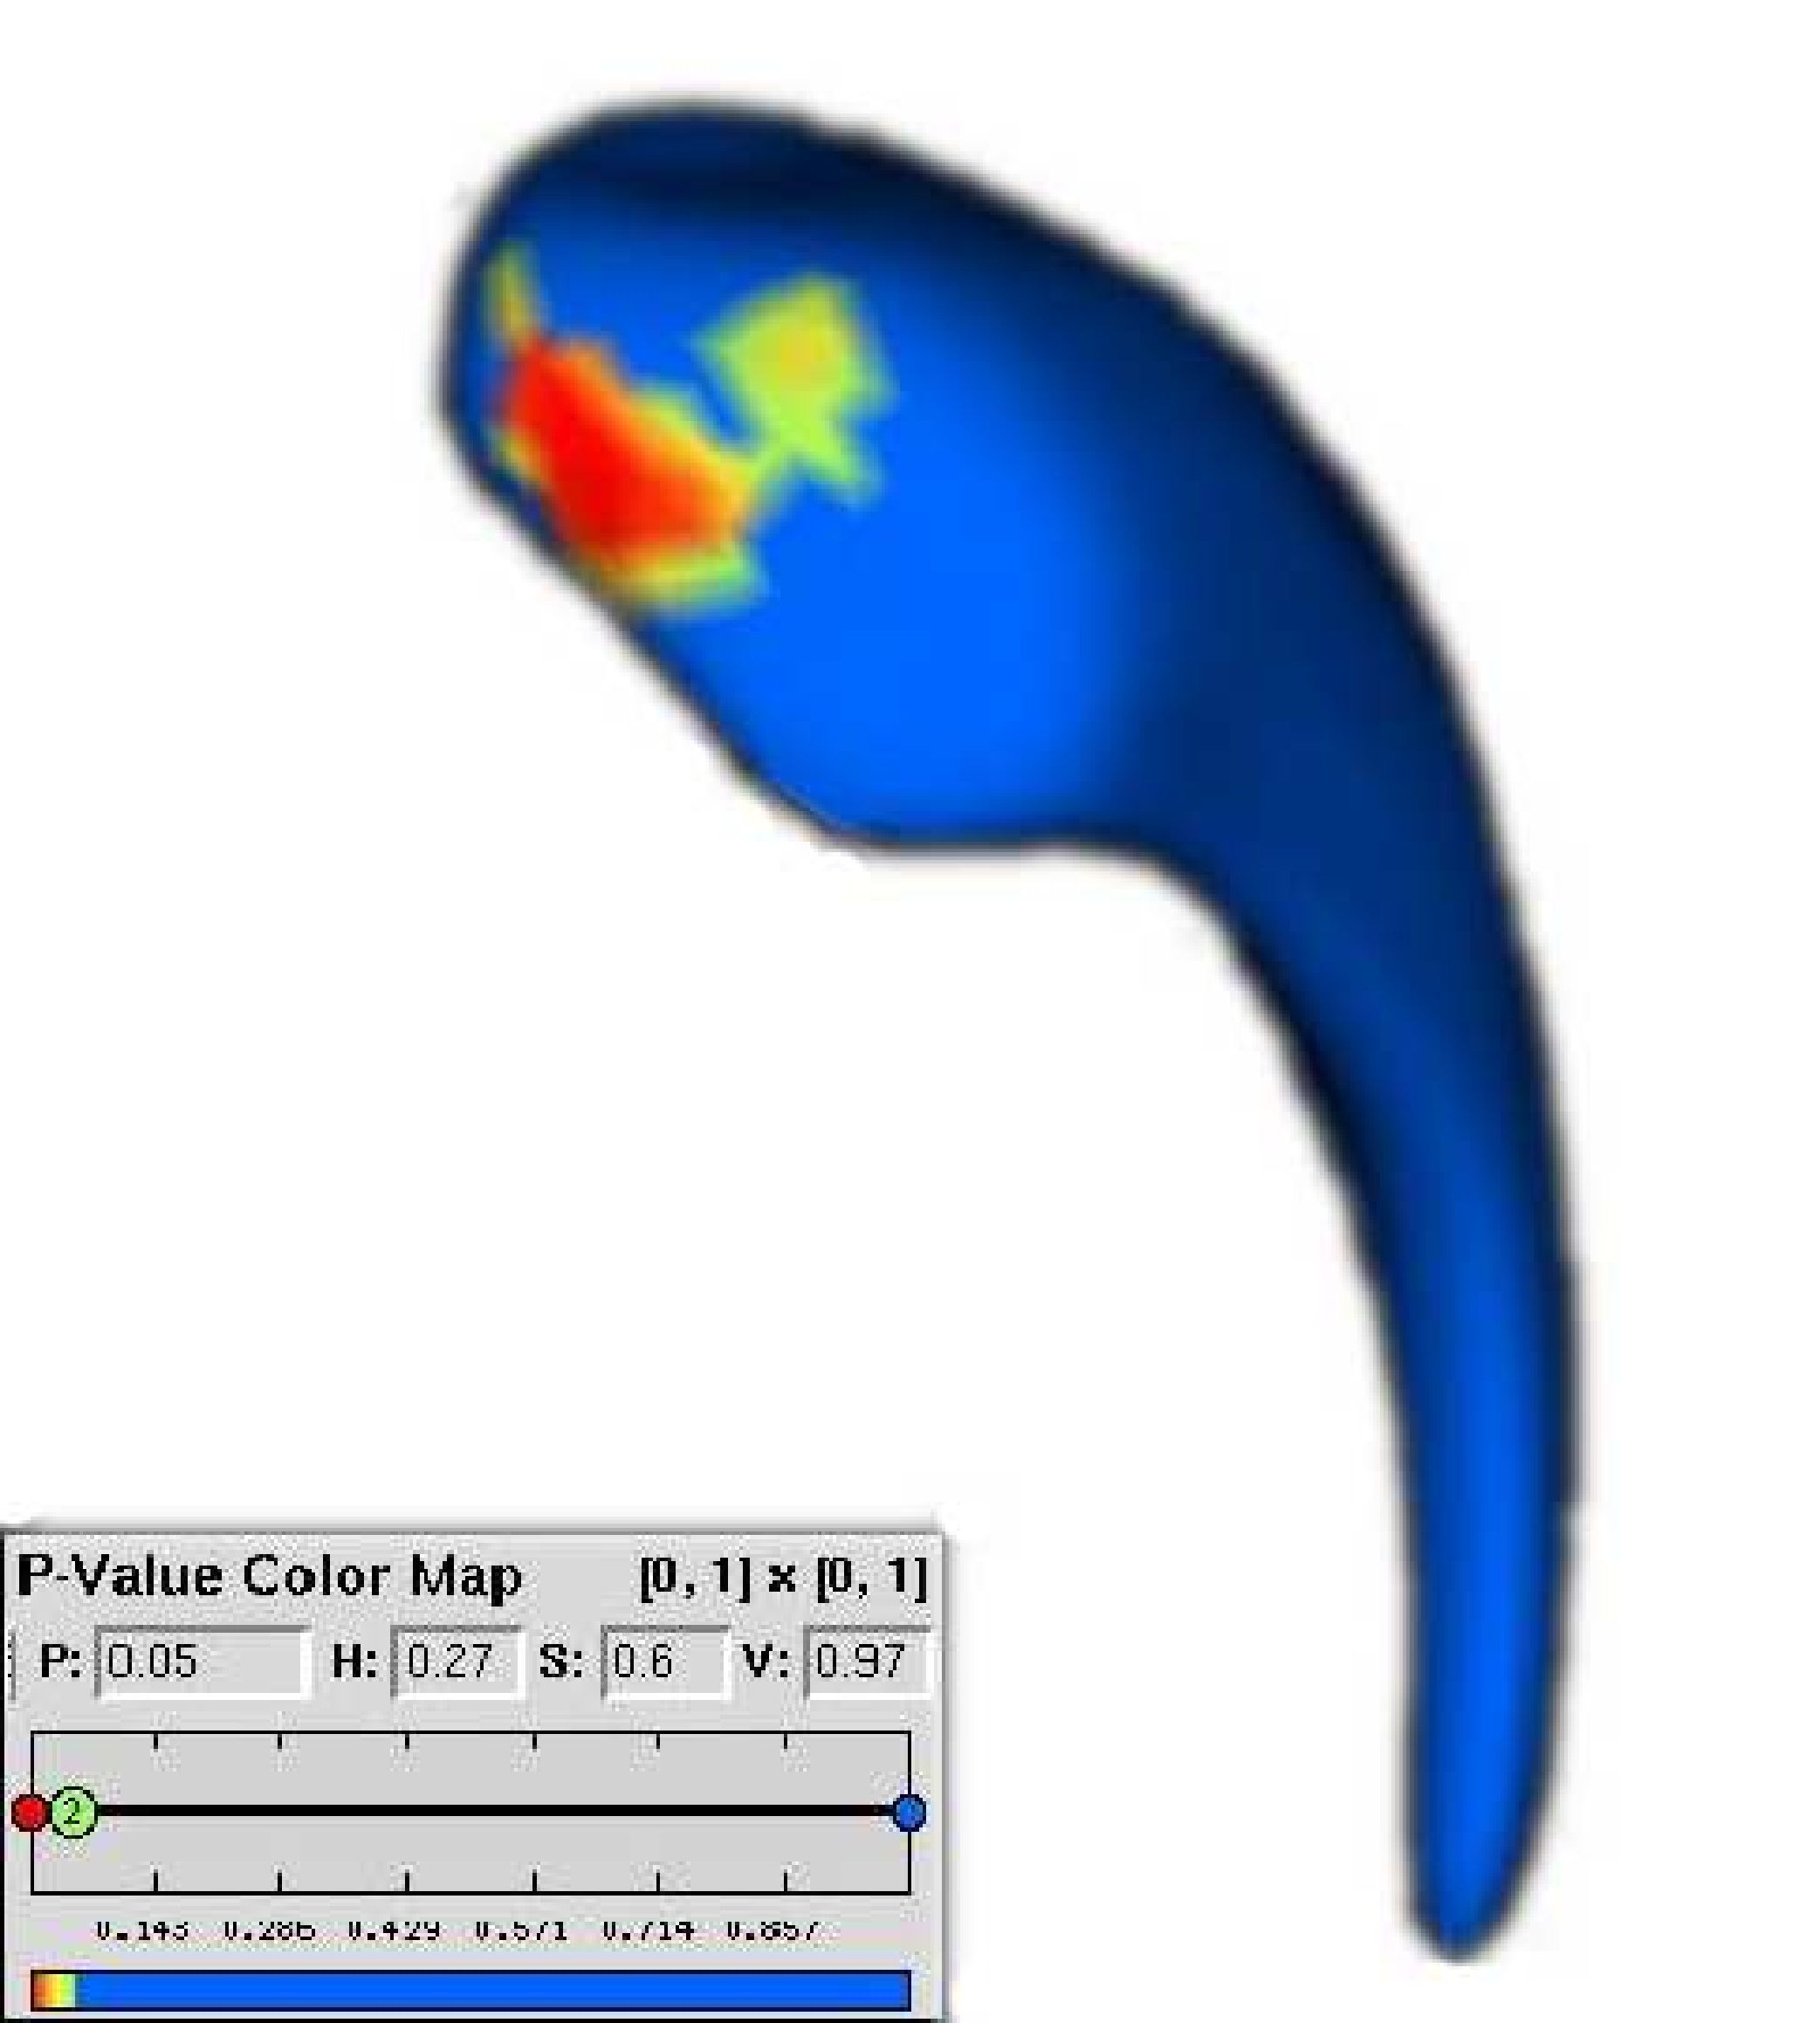
\includegraphics[width=6cm]{IJ_AnalysisScenario1_Correlations}
    \end{tabular}
    \itkcaption{Left: The raw p-values show that there is significant local shape difference mainly in the head of the caudate. Right: The raw p-values show that there is significant local shape correlation with the overall behavioral score, mainly in the head of the caudate.}
    \label{fig:rawP}
  \end{center}
\end{figure}

\subsection{Longitudinal groupwise analysis scenario}
\label{sec:results2}

In addition to groupwise analysis, \ProgramName also allows to test for differences between the surfaces of two different time points screenings in case of a same patient. The results displayed in this section are part of a schizophrenia study, and tries to find differences among subjects that progressed to schizophrenia and subjects that did not progress from the prodromal state using analysis of covariance. This analytic approach was used first for paired longitudinal comparisons between the baseline measurement and the subsequent follow-up measurements of the same patient. Three features were obtained from that analysis, all them based in the shape differences between the baseline and the follow up status of each subject: direction and magnitude of shape changes, as well as the associated statistical significance. The next step consisted in finding differences between groups of the previously computed features, in a similar fashion than in \ref{sec:results}. 

\subsubsection{Results}
\label{sec:lilresults2}

Visualization of the results obtained from the aforementioned tests (figures  \ref{fig:diff} - \ref{fig:pvals}) provide three kinds of information at a specific location on the surface:
	
\begin{itemize}
	\item Average magnitude and direction of the shape changes between progressers and non-progressers for schizophrenia: White color is used where the magnitudes are zero. The color gets darker as the magnitudes of the distance increase. The distance is positive if the mean surface of group A (progressers) is protruding outside of the mean surface of group B (non-progressers); the distance is negative if the mean surface of group A is shrinking below the mean surface of group B. Positive distances are color-coded by blue and negative distances are color-coded by red. (Figure \ref{fig:diff})
	\item Directionality of the shape changes: Displayed by means of vector maps that show the shape differences between the mean shape of the two groups tested. (Figure \ref{fig:vectors})
	\item Significance maps: Showing the areas in where the shape changes were considered to be statistically significant. The p-values are color-coded showing blue where the raw p-value exceeds 0.05, that is to say the change for that point is not significant regardless the magnitude of it, and red in those points where the changes are significant. (Figure \ref{fig:pvals})
\end{itemize}

\begin{figure}[htbp]
  \begin{center}
    \begin{tabular}[htbp]{c}
    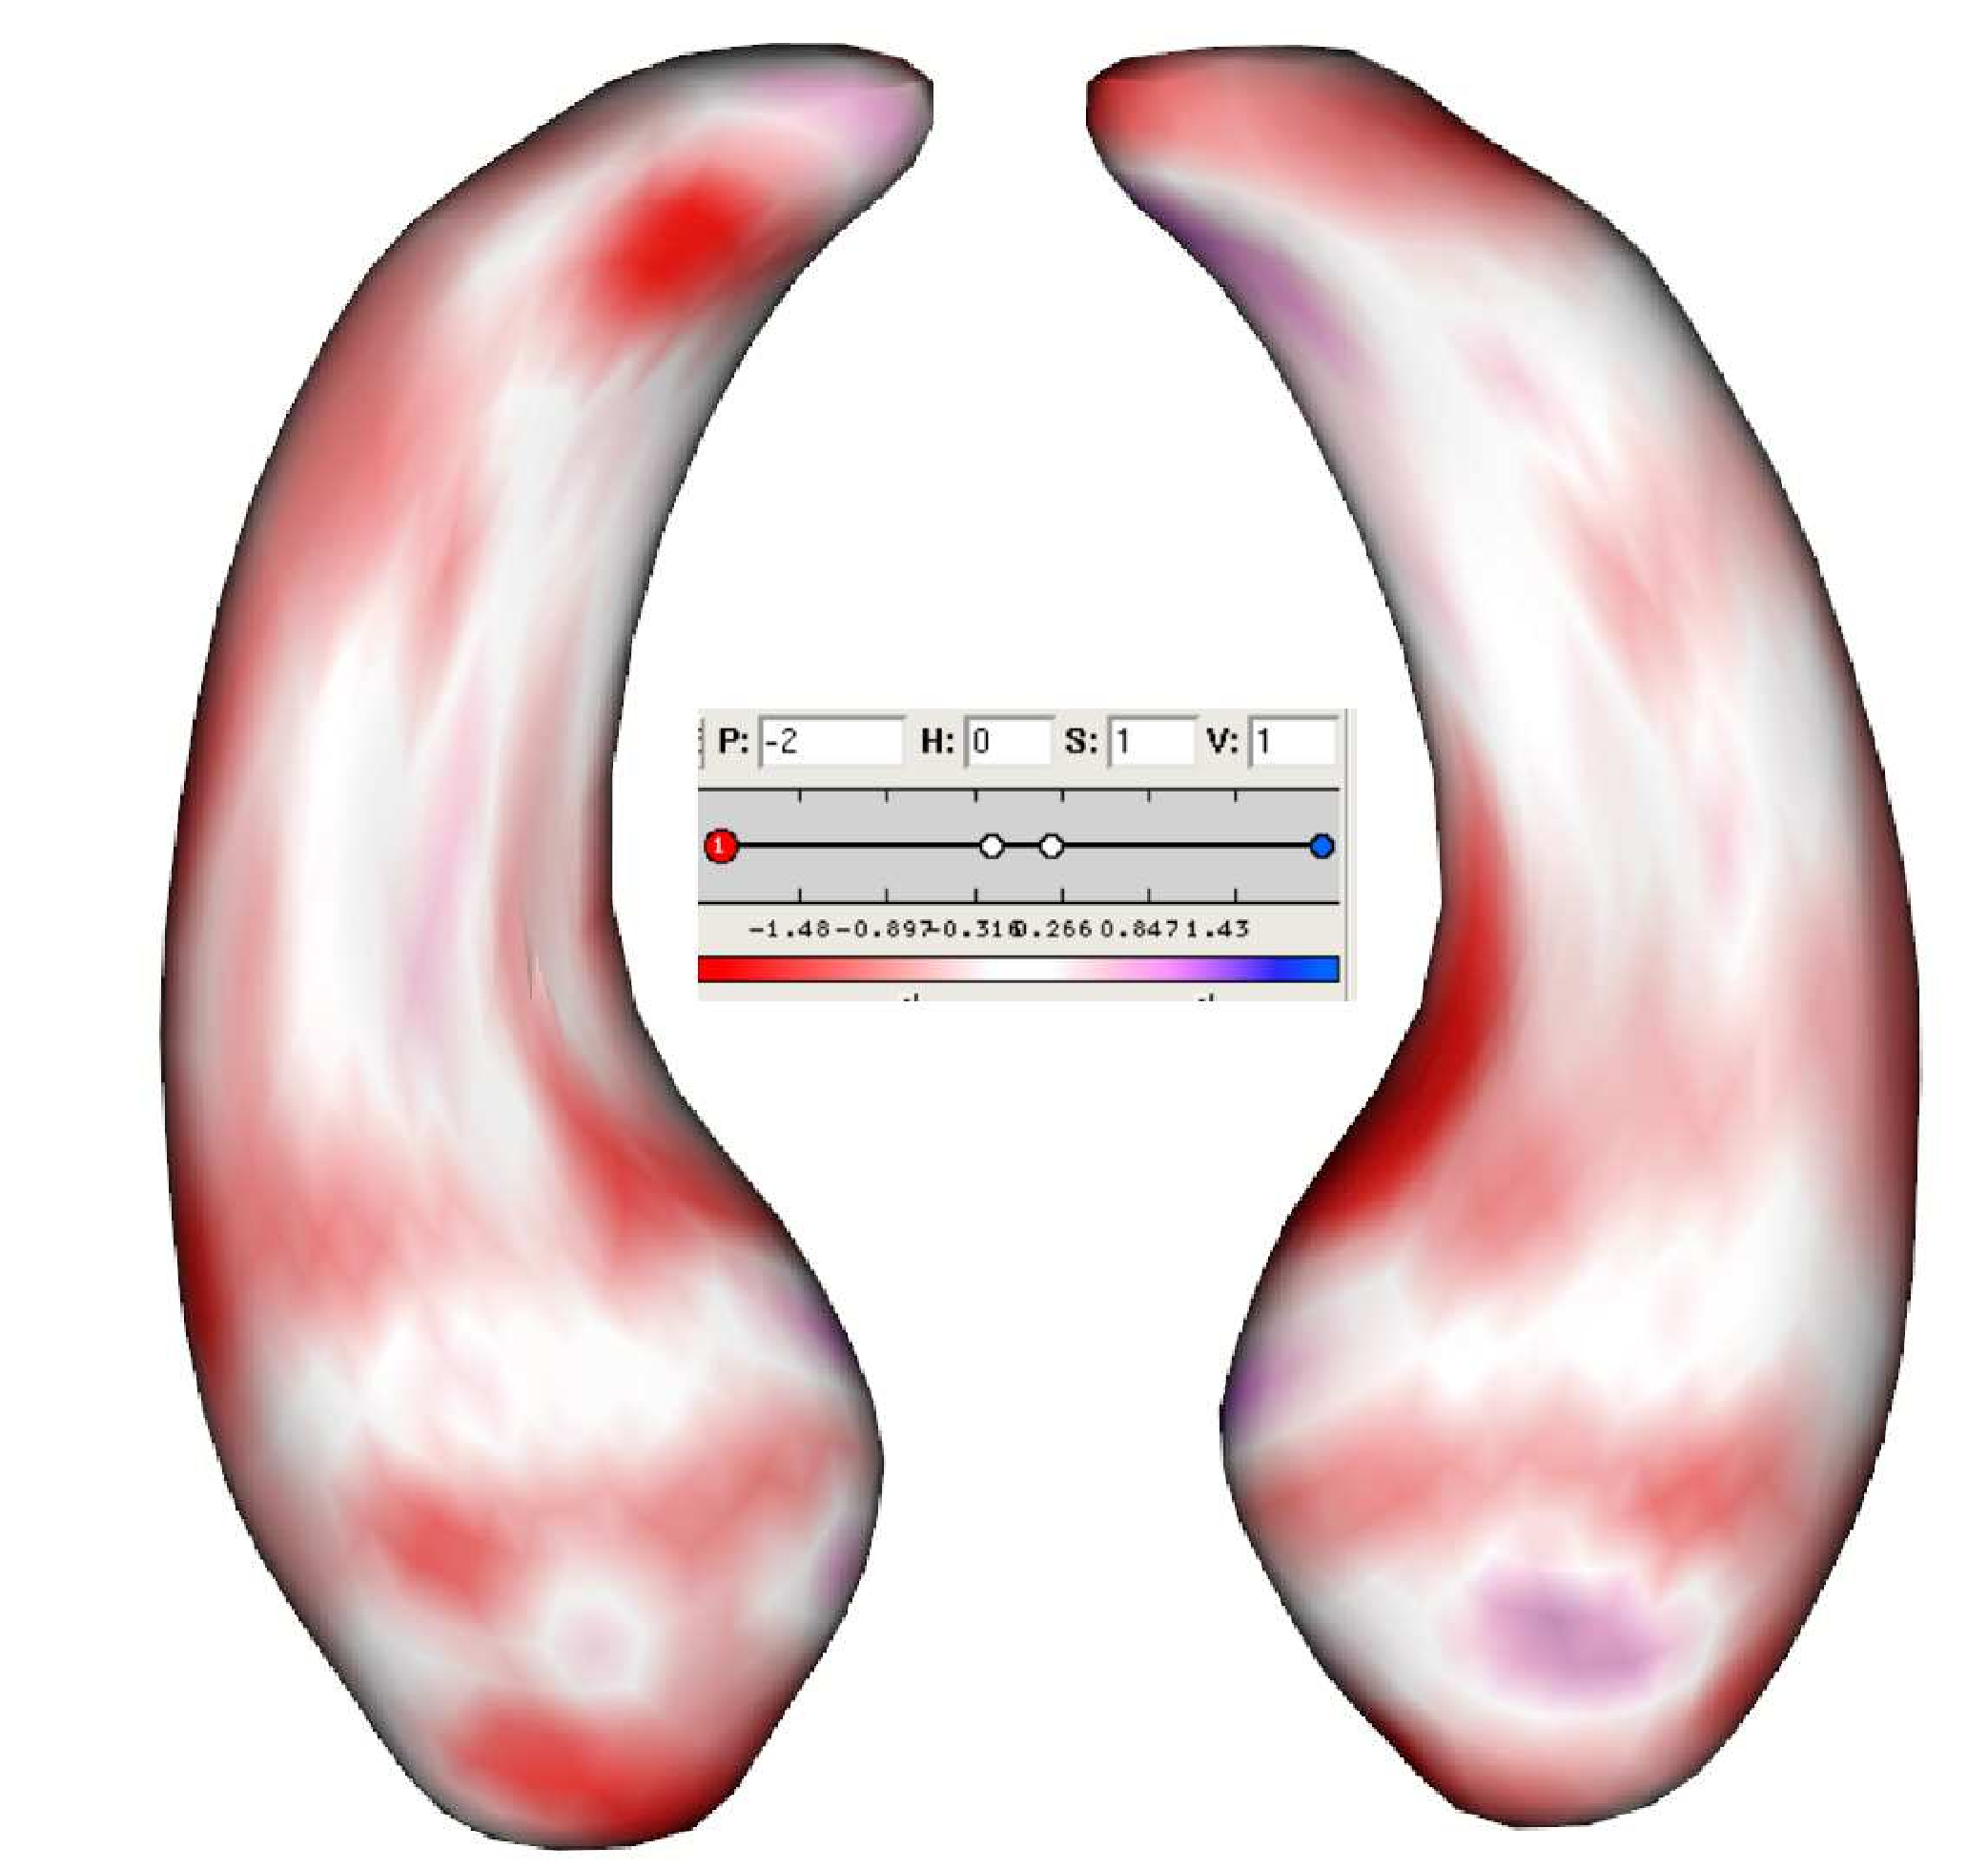
\includegraphics[width=0.6\textwidth]{IJ_AnalysisScenario2_MeanDiff}
    \end{tabular}
    \itkcaption{Magnitude and directional changes in hippocampus during the progression of schizophrenia.}
    \label{fig:diff}
  \end{center}
\end{figure}

\begin{figure}[htbp]
  \begin{center}
    \begin{tabular}[htbp]{c}
    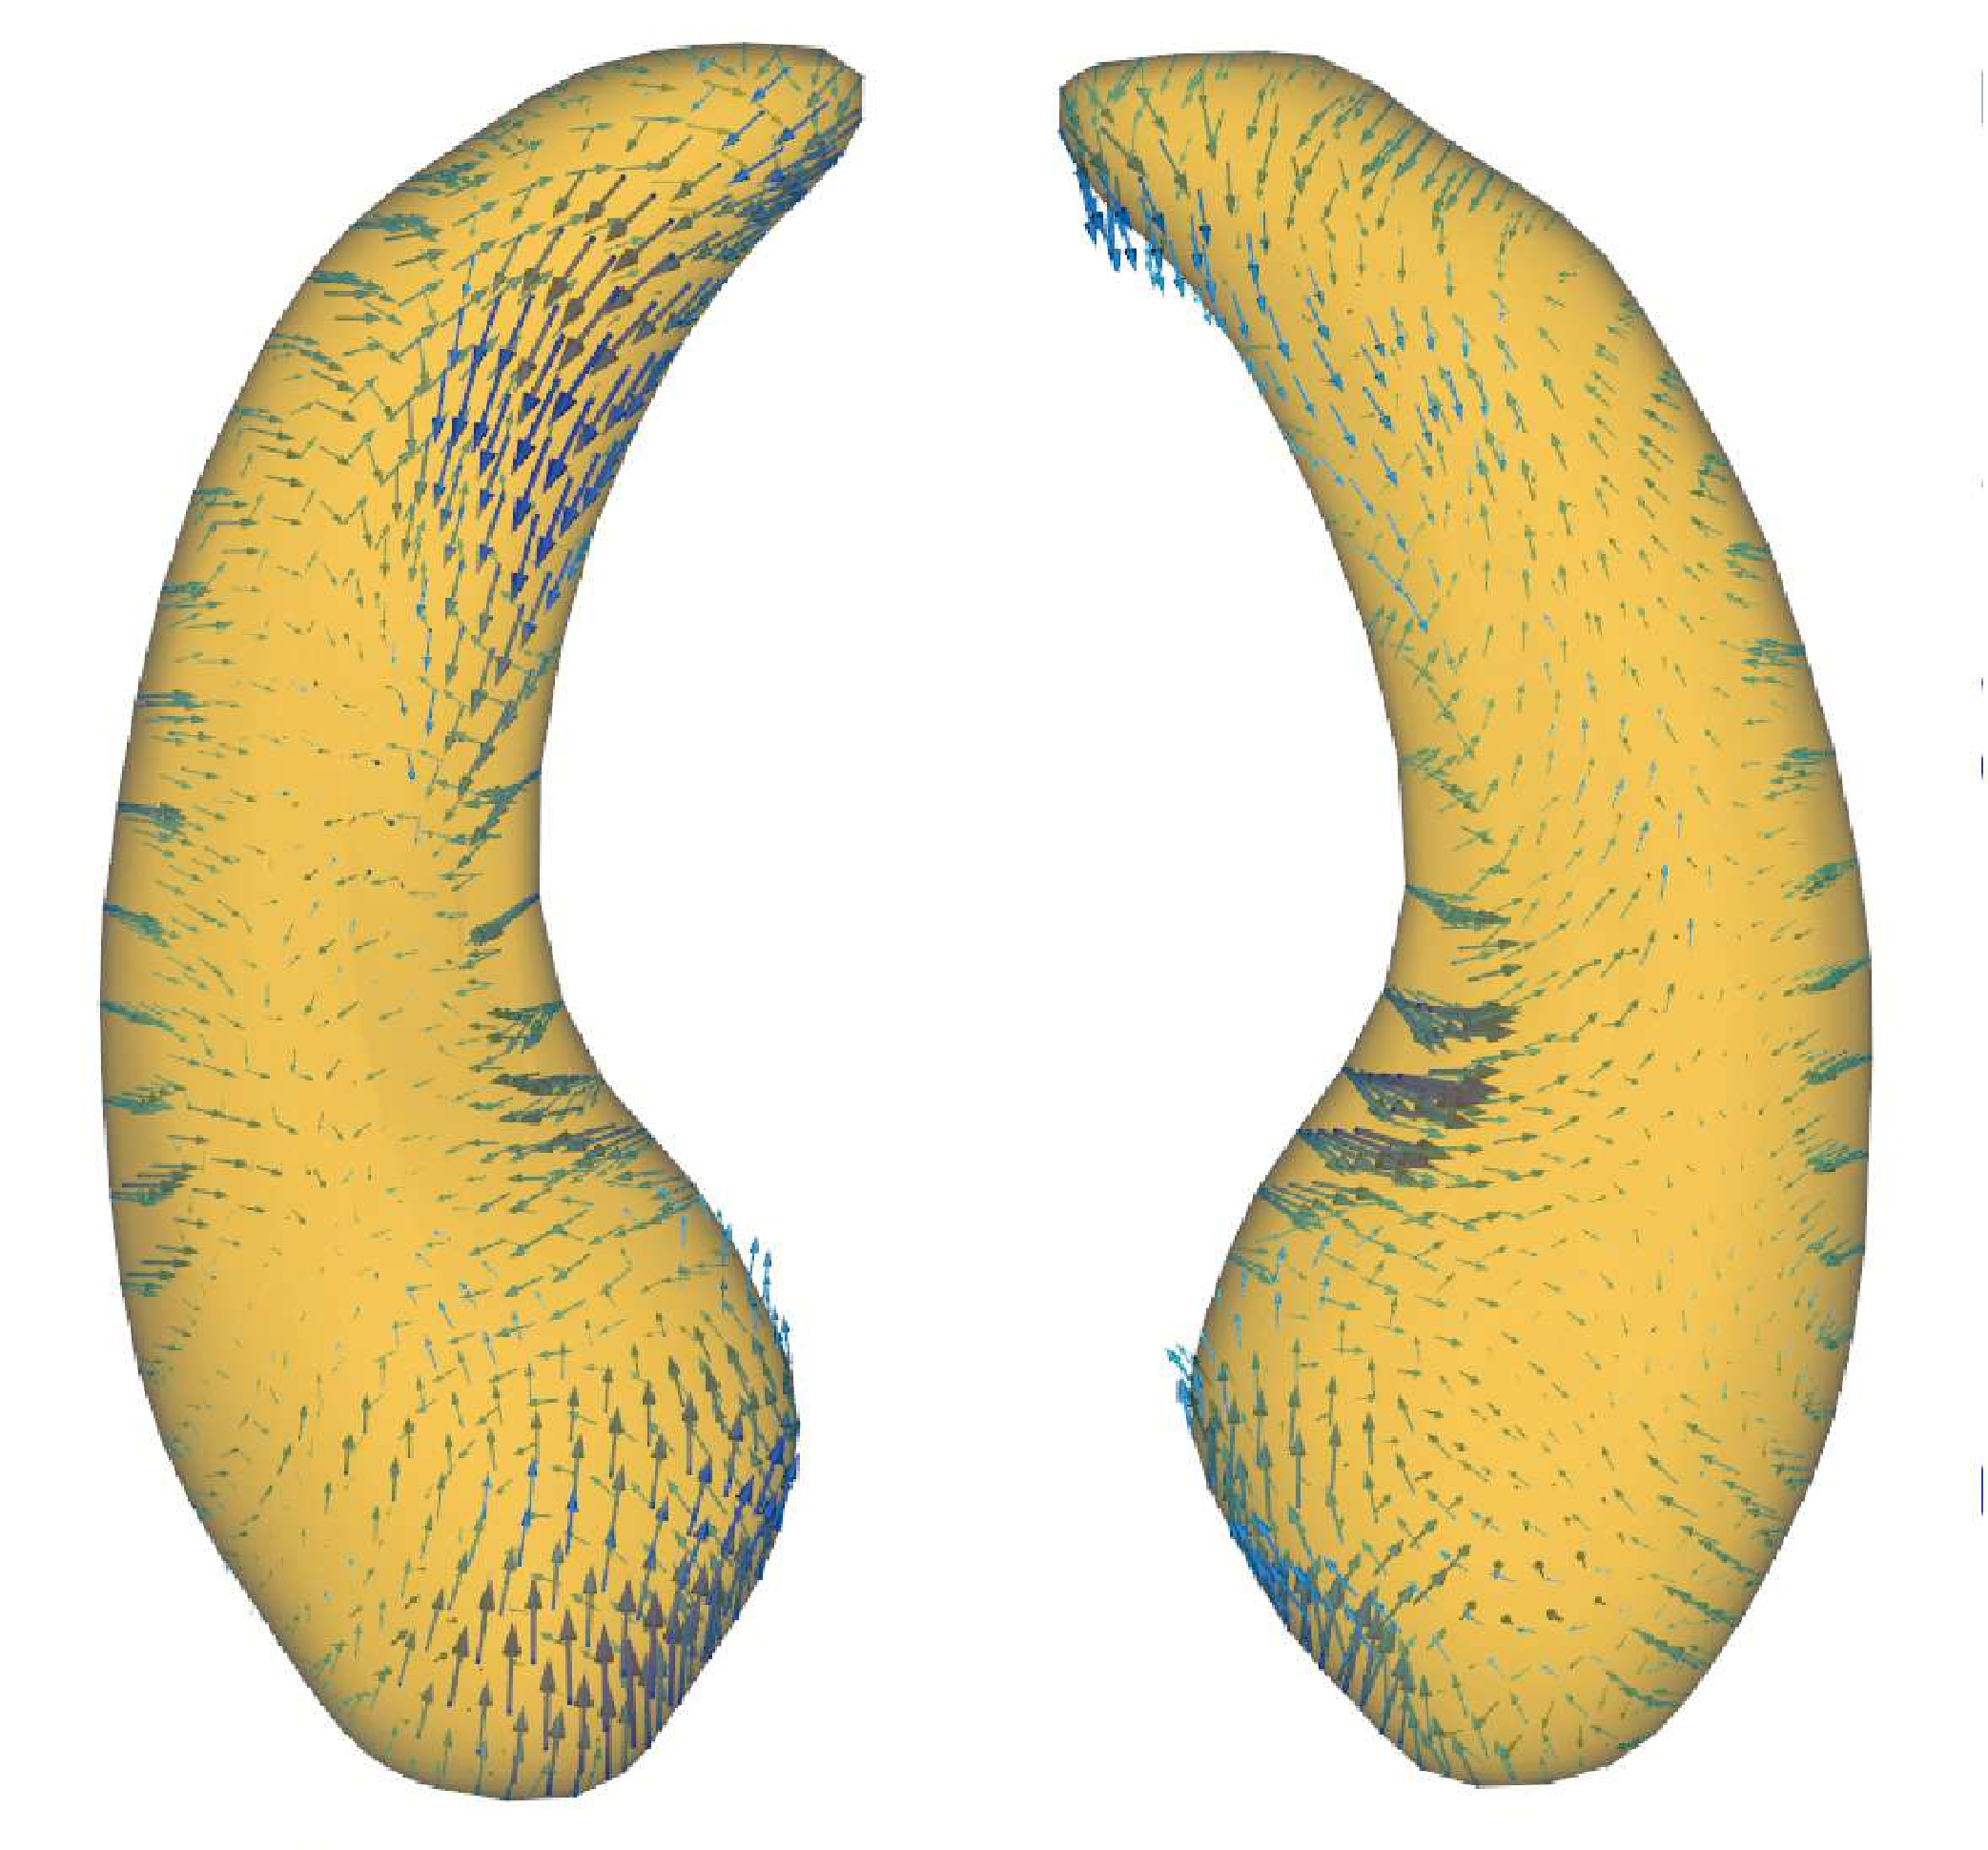
\includegraphics[width=0.6\textwidth]{IJ_AnalysisScenario2_Vectors}
    \end{tabular}
    \itkcaption{Directionality of shape changes displayed with vector maps.}
    \label{fig:vectors}
  \end{center}
\end{figure}

\begin{figure}[htbp]
  \begin{center}
    \begin{tabular}[htbp]{c}
    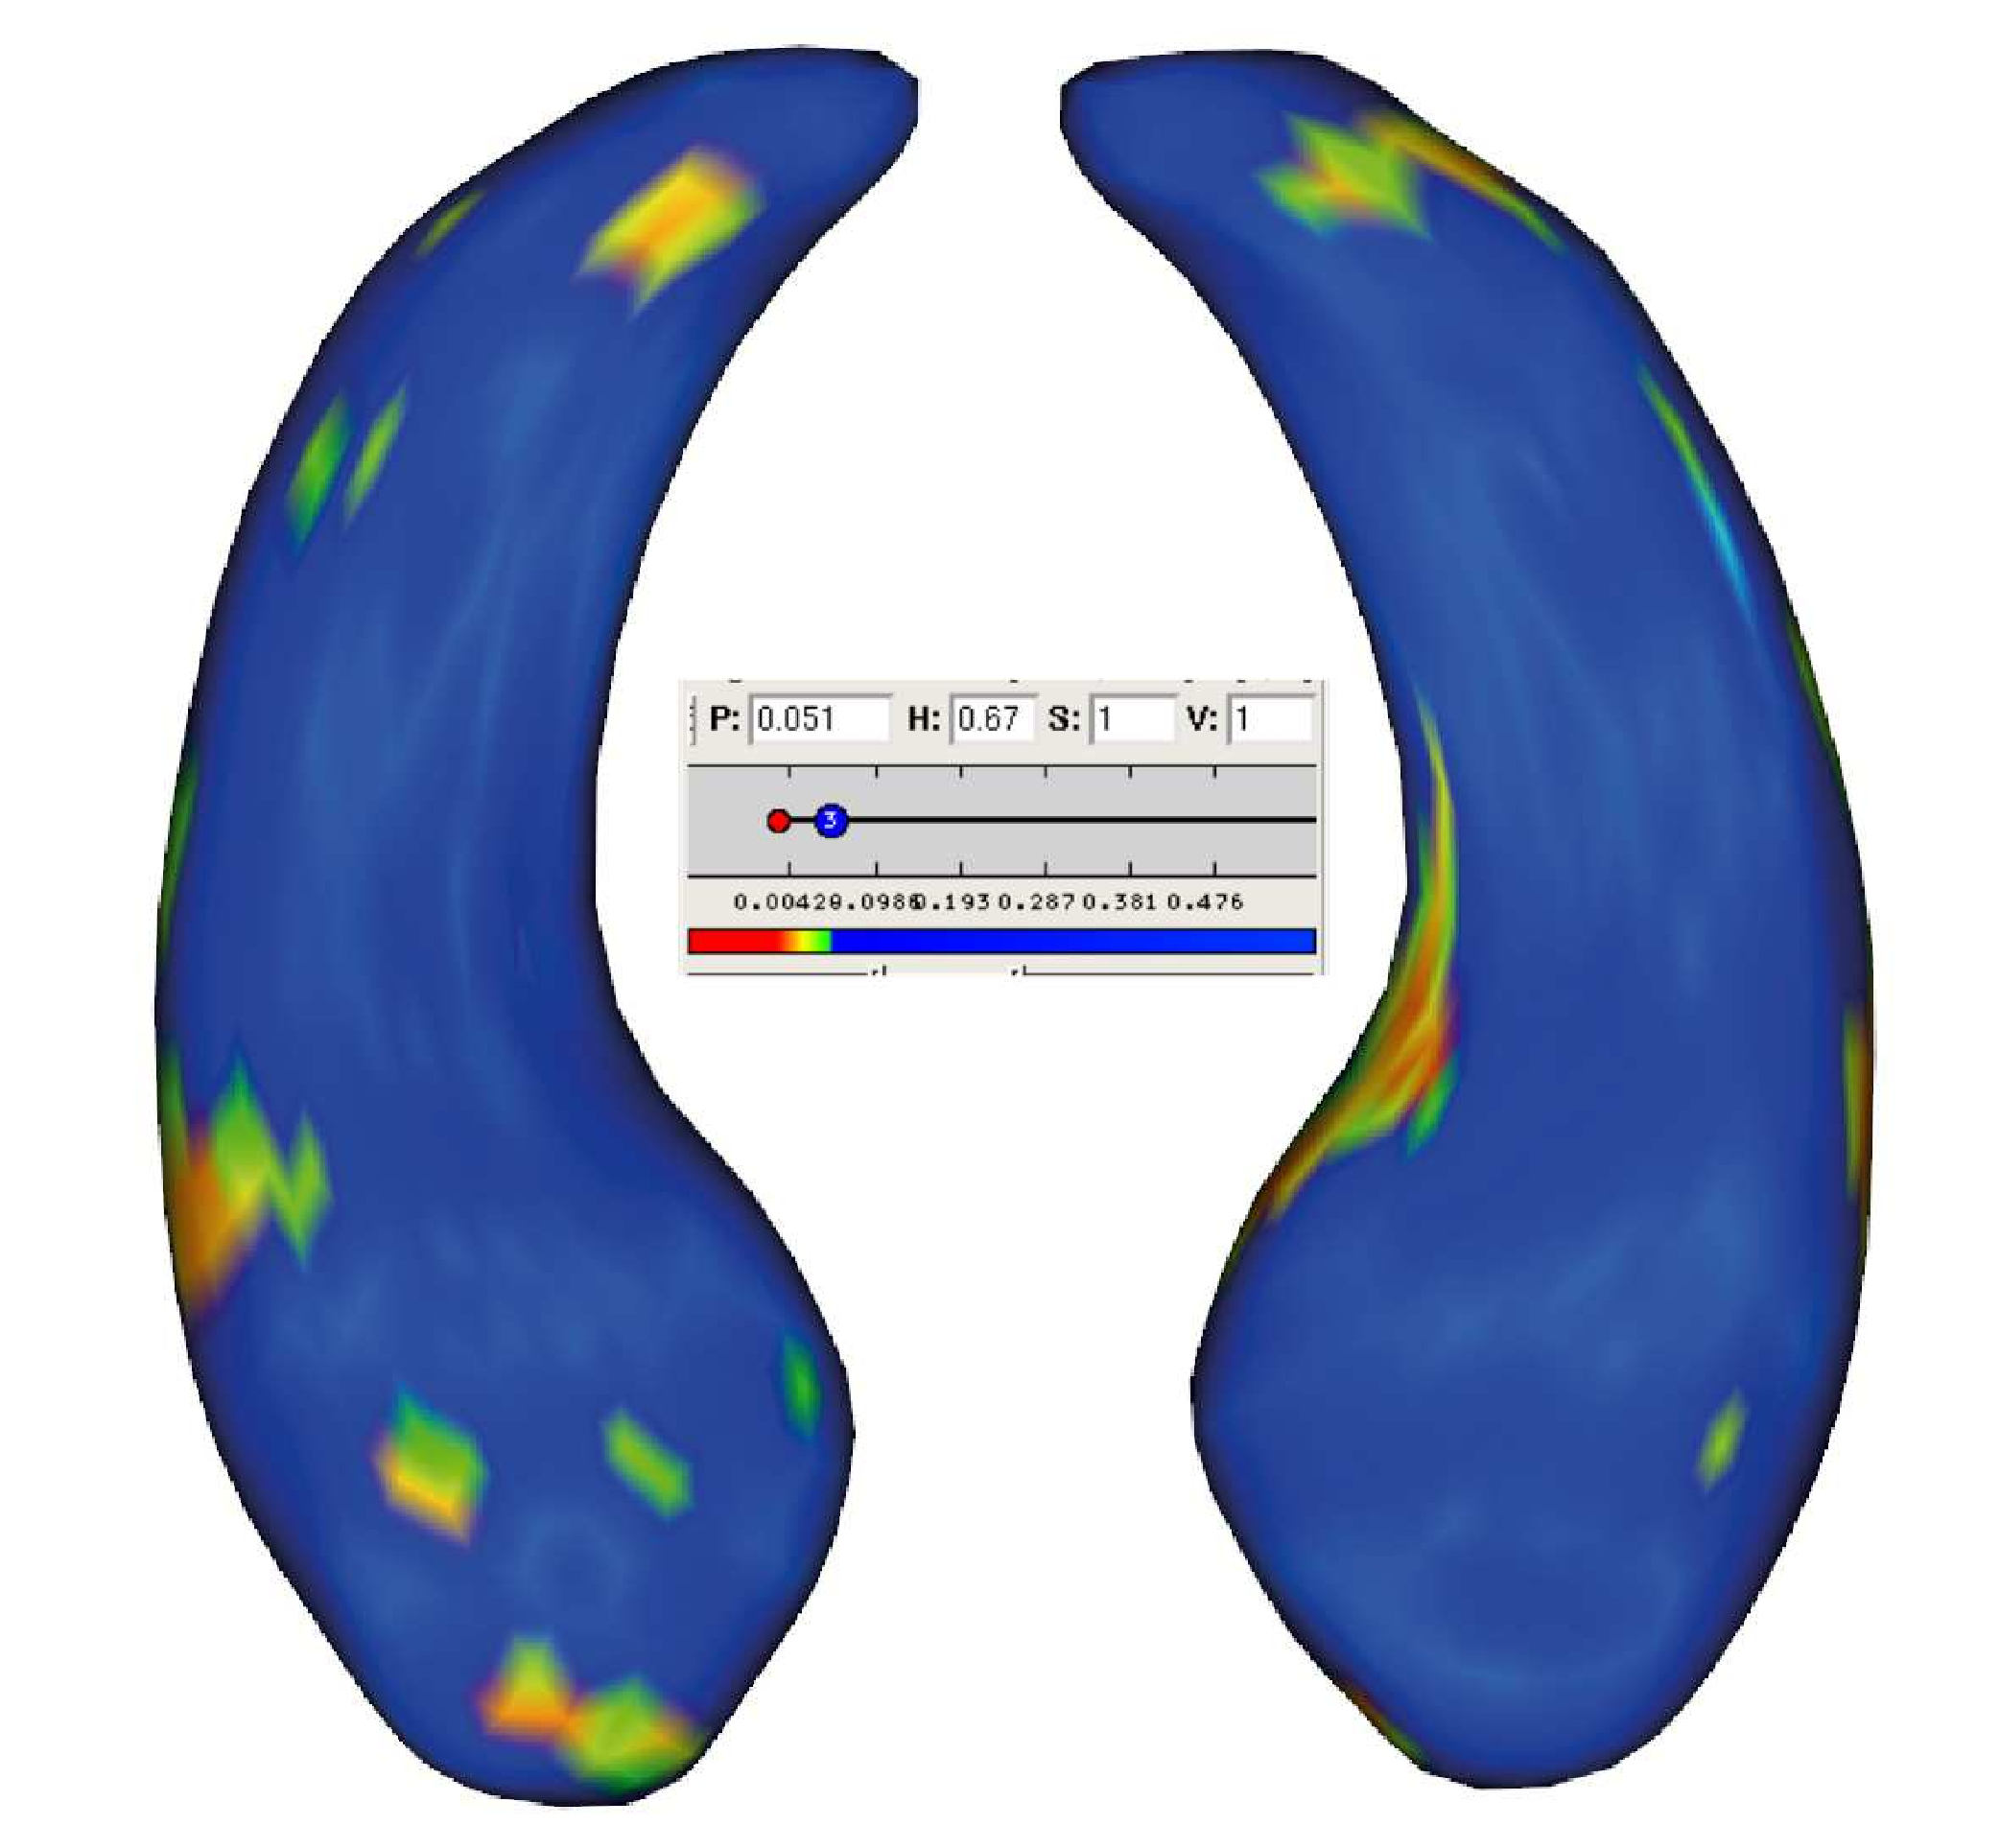
\includegraphics[width=0.6\textwidth]{IJ_AnalysisScenario2_RawPValues}
    \end{tabular}
    \itkcaption{Statistical significance for the shape changes in hippocampus during the progression of schizophrenia.}
    \label{fig:pvals}
  \end{center}
\end{figure}

\subsection{Cross-sectional with interaction variables groupwise analysis scenario}
\label{sec:results3}

This study was performed to determine the condylar morphological variation of osteoarthritic (OA) and asymptomatic temporomandibular joints (TMJ) and to determine its correlation with clinical signs and symptoms presented in the progression of the OA disease. The spectrum of clinical and pathological presentation of TMJ OA range from structural and functional failure of the joint with disc displacement and degeneration, to subchondral bone alterations (erosions), bone overgrowth (osteophytes), loss of articular fibrocartilage, and synovitis. Many osteoarthritic TMJs are associated with clinical symptoms \cite{Hatcher91} \cite{Helenius05}. However, some are completely asymptomatic. The factor(s) which relates the morphological changes and clinical signs and symptoms (namely pain, joint sounds, and mandibular range of motion) is unknown.  

Preliminary findings in this field were obtained using \ProgramName, computing Pearson correlation coefficients and their p-values between morphological variation and clinical variables for a dataset of 29 female patients with TMJ OA (Research Diagnostic Criteria for Temporomandibular Disorders Group III) and 40 female asymptomatic subjects. In this analysis scenario only results for correlations pain onset will be displayed, and were obtained with the following sequence of arguments,

Example command: `\program infile - -numGroupTypes 1 - -numIndependent 1 - -interactionTest - -simpleCorrs'

\subsubsection{Results}
\label{sec:lilresults3}

In the Pearson correlation coefficient maps, positive correlations are color-coded red and negative correlations are green. Yellow is used where there are no relevant correlation between shape and pain onset (coefficients equals or close to zero) P-values maps show the associated statistical significance for the correlation coefficients previously described. In the p-values maps very high correlations ($p < 0.01$) are color-coded with white, significant correlations are color-coded with red and green ($0.01 > p > 0.05$) and no significant correlations are color-coded with blue. The results for correlations between shape changes and pain onset are shown in figure \ref{fig:pearson}.

\begin{figure}[htbp]
  \begin{center}
    \begin{tabular}[htbp]{c}
    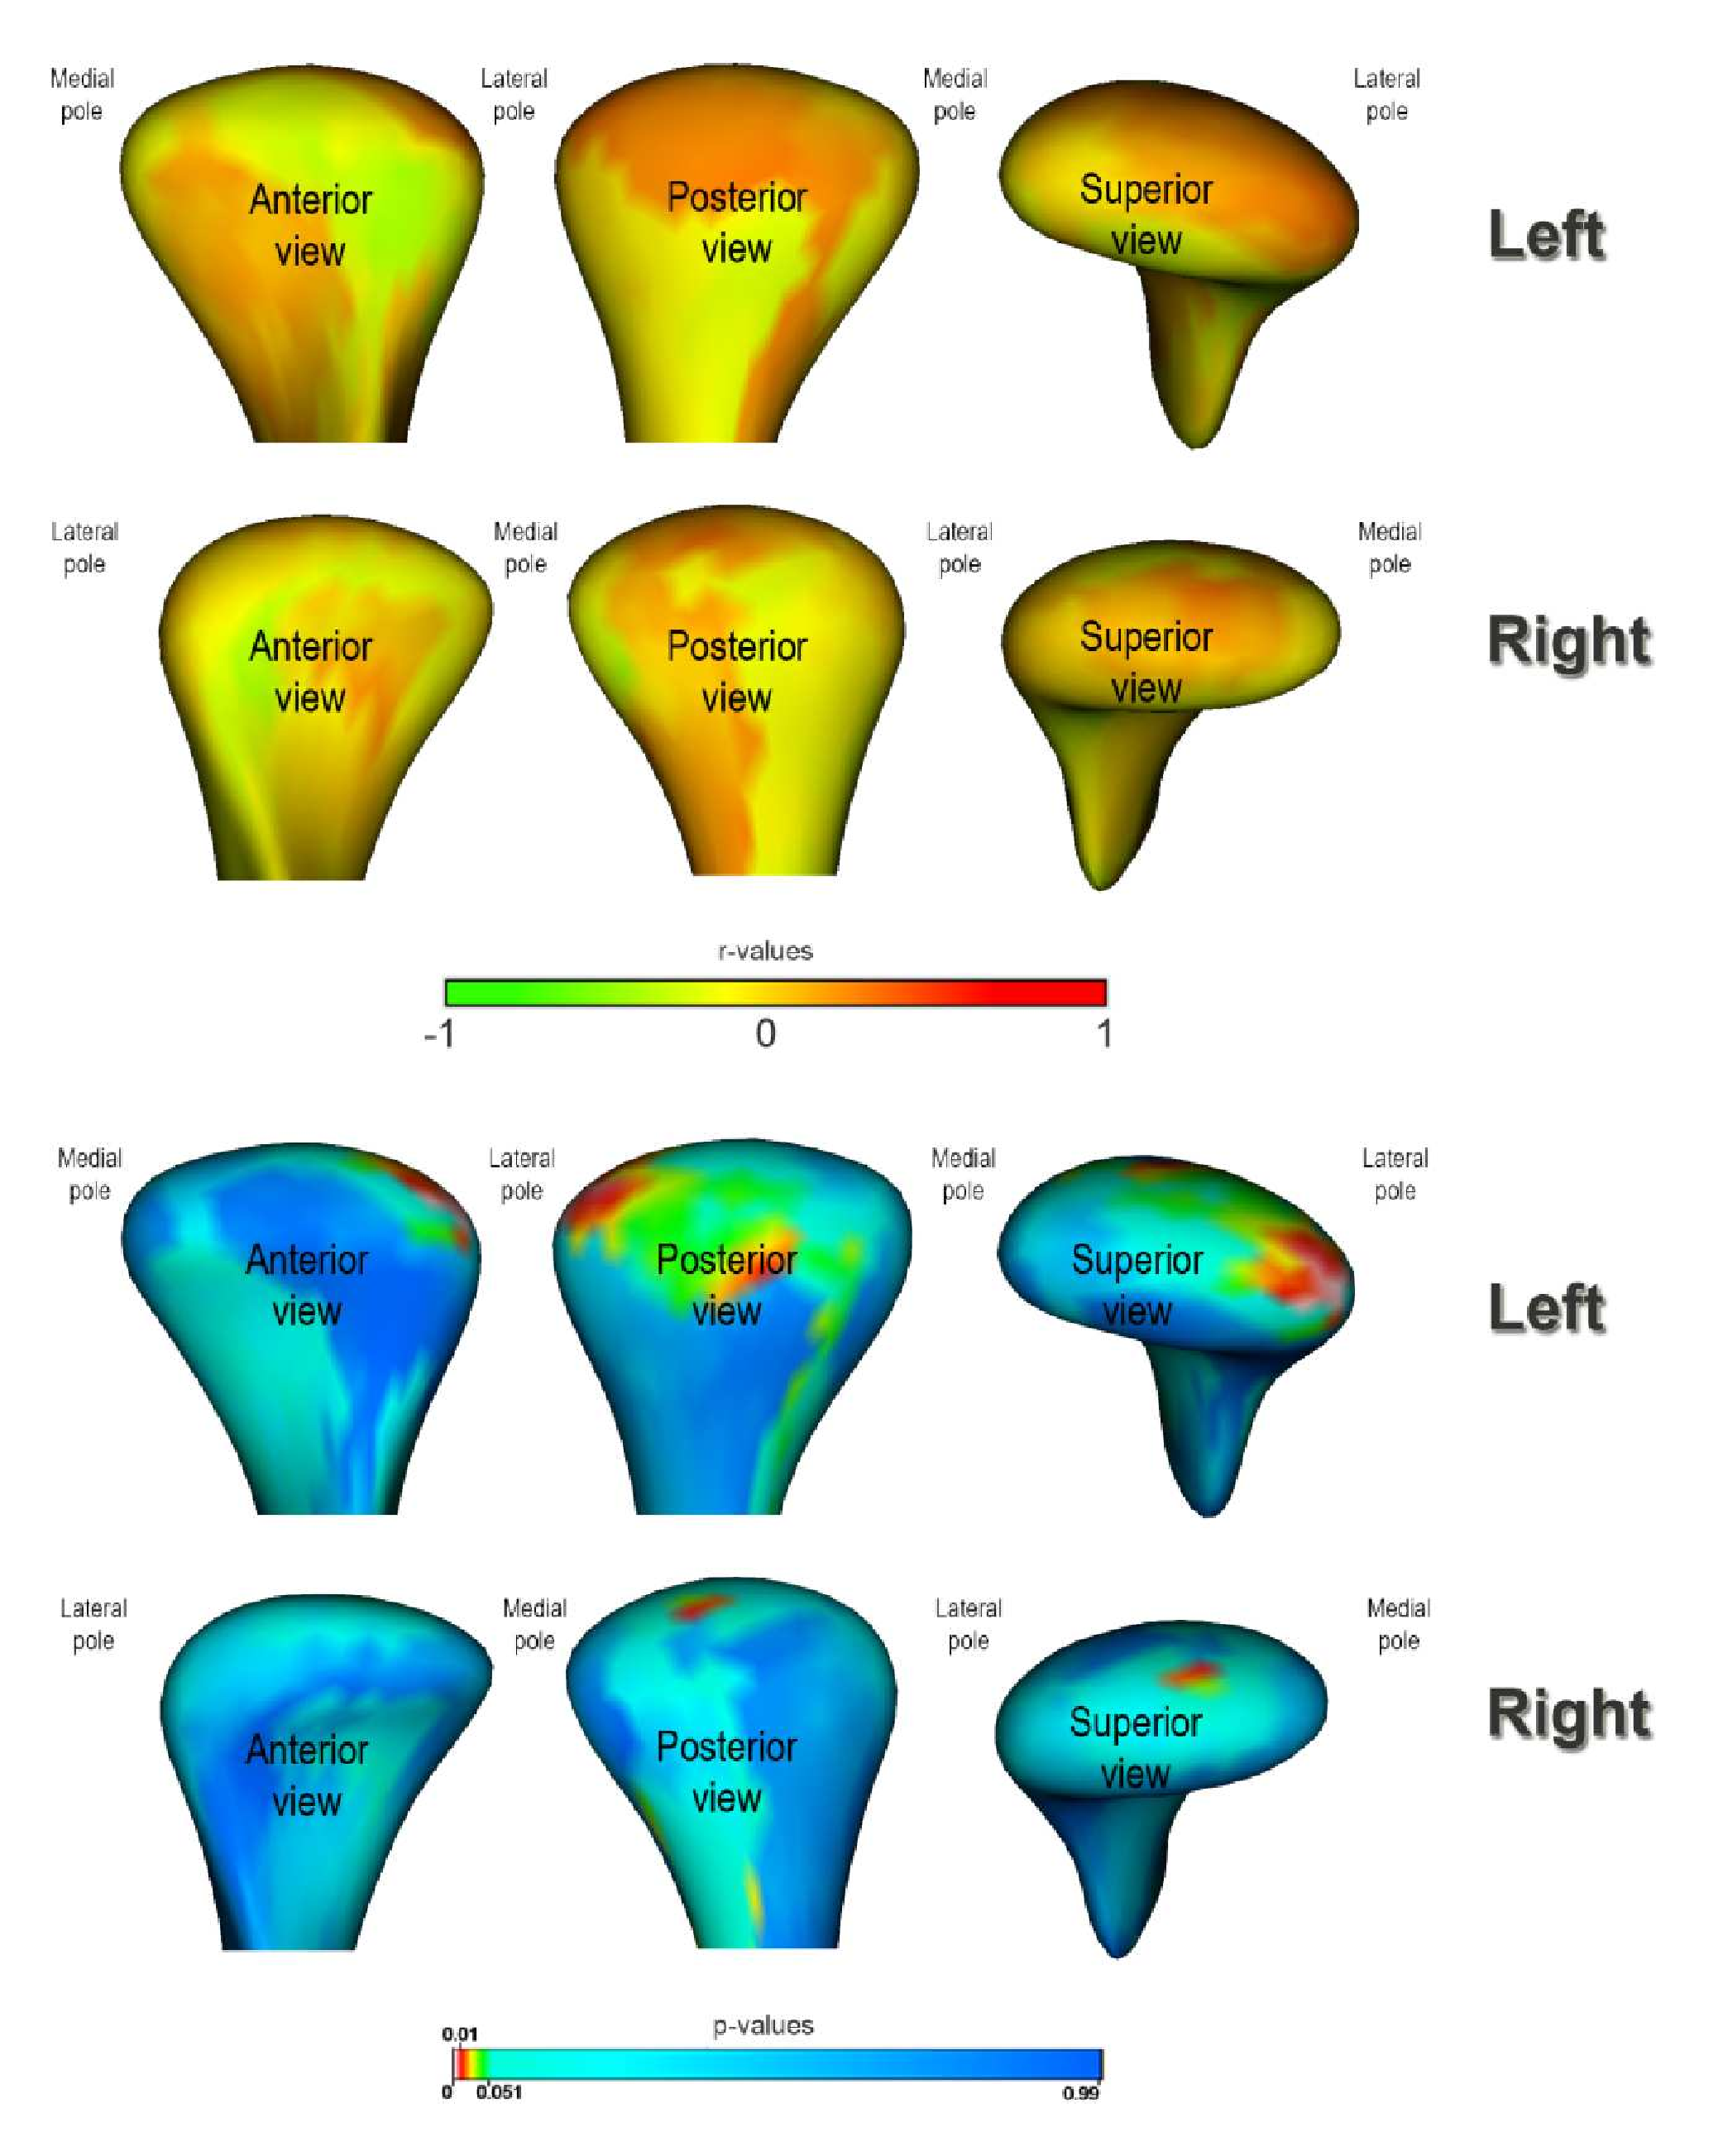
\includegraphics[width=0.8\textwidth]{IJ_AnalysisScenario3_Correlations}
    \end{tabular}
    \itkcaption{Morphological correlation with pain variables (pain onset).  Up, Pearson correlation coefficients. Down, associated statistical significance maps. The significance maps show statistically significant correlations in the the lateral and posterior surfaces of the condyles.}
    \label{fig:pearson}
  \end{center}
\end{figure}

\section{Conclusions}
\label{sec:conclusions}
We presented a novel statistical shape analysis tool called \ProgramName. The versatility of the tool allows it to be applied in many different shape morphometry applications. This paper described the methodology associated with the tool as well as a set of case studies in shape analysis. We are currently applying this tool in our studies of shape in schizophrenia, autism, TMJ and normal development. 

\section*{Acknowledgements}

This work was supported by grants from the NIDCR (DE018962), NAMIC (U54 EB005149) and NDRC (UNC P30 HD03110). Many thanks to the departments of Neurology and Psychiatry from Columbia University, and specially to Scott Schobel for providing the data presented in the Longitudinal groupwise analysis scenario (section \ref{sec:results2}).

%%%%%%%%%%%%%%%%%%%%%%%%%%%%%%%%%%%%%%%%%
%
%  Insert the bibliography using BibTeX
%
%%%%%%%%%%%%%%%%%%%%%%%%%%%%%%%%%%%%%%%%%

\bibliographystyle{plain}
\bibliography{Mybib}


\end{document}

